\documentclass[twoside]{article}

% Packages required by doxygen
\usepackage{fixltx2e}
\usepackage{calc}
\usepackage{doxygen}
\usepackage[export]{adjustbox} % also loads graphicx
\usepackage{graphicx}
\usepackage[utf8]{inputenc}
\usepackage{makeidx}
\usepackage{multicol}
\usepackage{multirow}
\PassOptionsToPackage{warn}{textcomp}
\usepackage{textcomp}
\usepackage[nointegrals]{wasysym}
\usepackage[table]{xcolor}

% Font selection
\usepackage[T1]{fontenc}
\usepackage[scaled=.90]{helvet}
\usepackage{courier}
\usepackage{amssymb}
\usepackage{sectsty}
\renewcommand{\familydefault}{\sfdefault}
\allsectionsfont{%
  \fontseries{bc}\selectfont%
  \color{darkgray}%
}
\renewcommand{\DoxyLabelFont}{%
  \fontseries{bc}\selectfont%
  \color{darkgray}%
}
\newcommand{\+}{\discretionary{\mbox{\scriptsize$\hookleftarrow$}}{}{}}

% Page & text layout
\usepackage{geometry}
\geometry{%
  a4paper,%
  top=2.5cm,%
  bottom=2.5cm,%
  left=2.5cm,%
  right=2.5cm%
}
\tolerance=750
\hfuzz=15pt
\hbadness=750
\setlength{\emergencystretch}{15pt}
\setlength{\parindent}{0cm}
\setlength{\parskip}{0.2cm}
\makeatletter
\renewcommand{\paragraph}{%
  \@startsection{paragraph}{4}{0ex}{-1.0ex}{1.0ex}{%
    \normalfont\normalsize\bfseries\SS@parafont%
  }%
}
\renewcommand{\subparagraph}{%
  \@startsection{subparagraph}{5}{0ex}{-1.0ex}{1.0ex}{%
    \normalfont\normalsize\bfseries\SS@subparafont%
  }%
}
\makeatother

% Headers & footers
\usepackage{fancyhdr}
\pagestyle{fancyplain}
\fancyhead[LE]{\fancyplain{}{\bfseries\thepage}}
\fancyhead[CE]{\fancyplain{}{}}
\fancyhead[RE]{\fancyplain{}{\bfseries\leftmark}}
\fancyhead[LO]{\fancyplain{}{\bfseries\rightmark}}
\fancyhead[CO]{\fancyplain{}{}}
\fancyhead[RO]{\fancyplain{}{\bfseries\thepage}}
\fancyfoot[LE]{\fancyplain{}{}}
\fancyfoot[CE]{\fancyplain{}{}}
\fancyfoot[RE]{\fancyplain{}{\bfseries\scriptsize Generated on Thu Oct 1 2015 12\+:42\+:35 for M\+E\+M\+O\+R\+Y M\+A\+N\+A\+G\+E\+M\+E\+N\+T by Doxygen }}
\fancyfoot[LO]{\fancyplain{}{\bfseries\scriptsize Generated on Thu Oct 1 2015 12\+:42\+:35 for M\+E\+M\+O\+R\+Y M\+A\+N\+A\+G\+E\+M\+E\+N\+T by Doxygen }}
\fancyfoot[CO]{\fancyplain{}{}}
\fancyfoot[RO]{\fancyplain{}{}}
\renewcommand{\footrulewidth}{0.4pt}
\renewcommand{\sectionmark}[1]{%
  \markright{\thesection\ #1}%
}

% Indices & bibliography
\usepackage{natbib}
\usepackage[titles]{tocloft}
\setcounter{tocdepth}{3}
\setcounter{secnumdepth}{5}
\makeindex

% Hyperlinks (required, but should be loaded last)
\usepackage{ifpdf}
\ifpdf
  \usepackage[pdftex,pagebackref=true]{hyperref}
\else
  \usepackage[ps2pdf,pagebackref=true]{hyperref}
\fi
\hypersetup{%
  colorlinks=true,%
  linkcolor=blue,%
  citecolor=blue,%
  unicode%
}

% Custom commands
\newcommand{\clearemptydoublepage}{%
  \newpage{\pagestyle{empty}\cleardoublepage}%
}


%===== C O N T E N T S =====

\begin{document}

% Titlepage & ToC
\hypersetup{pageanchor=false,
             bookmarks=true,
             bookmarksnumbered=true,
             pdfencoding=unicode
            }
\pagenumbering{roman}
\begin{titlepage}
\vspace*{7cm}
\begin{center}%
{\Large M\+E\+M\+O\+R\+Y M\+A\+N\+A\+G\+E\+M\+E\+N\+T \\[1ex]\large version1 }\\
\vspace*{1cm}
{\large Generated by Doxygen 1.8.9.1}\\
\vspace*{0.5cm}
{\small Thu Oct 1 2015 12:42:35}\\
\end{center}
\end{titlepage}
\tableofcontents
\pagenumbering{arabic}
\hypersetup{pageanchor=true}

%--- Begin generated contents ---
\section{File Index}
\subsection{File List}
Here is a list of all files with brief descriptions\+:\begin{DoxyCompactList}
\item\contentsline{section}{lib/\hyperlink{memory_management_8h}{memory\+Management.\+h} }{\pageref{memory_management_8h}}{}
\item\contentsline{section}{src/\hyperlink{memory_management_8c}{memory\+Management.\+c} }{\pageref{memory_management_8c}}{}
\item\contentsline{section}{src/\hyperlink{user_8c}{user.\+c} }{\pageref{user_8c}}{}
\end{DoxyCompactList}

\section{File Documentation}
\hypertarget{memory_management_8h}{}\subsection{lib/memory\+Management.h File Reference}
\label{memory_management_8h}\index{lib/memory\+Management.\+h@{lib/memory\+Management.\+h}}
{\ttfamily \#include $<$stdio.\+h$>$}\\*
{\ttfamily \#include $<$stdlib.\+h$>$}\\*
{\ttfamily \#include $<$string.\+h$>$}\\*
{\ttfamily \#include $<$time.\+h$>$}\\*
Include dependency graph for memory\+Management.\+h\+:
\nopagebreak
\begin{figure}[H]
\begin{center}
\leavevmode
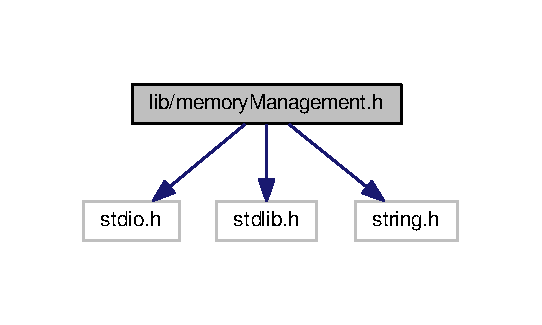
\includegraphics[width=322pt]{memory_management_8h__incl}
\end{center}
\end{figure}
This graph shows which files directly or indirectly include this file\+:
\nopagebreak
\begin{figure}[H]
\begin{center}
\leavevmode
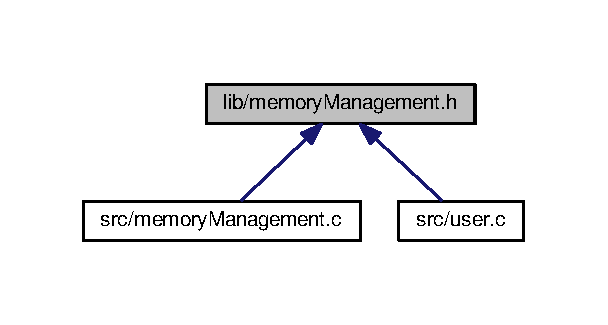
\includegraphics[width=292pt]{memory_management_8h__dep__incl}
\end{center}
\end{figure}
\subsubsection*{Macros}
\begin{DoxyCompactItemize}
\item 
\#define \hyperlink{memory_management_8h_a3018c7600b7bb9866400596a56a57af7}{S\+T\+A\+R\+T}~0
\item 
\#define \hyperlink{memory_management_8h_a70ed59adcb4159ac551058053e649640}{S\+I\+Z\+E}~1
\item 
\#define \hyperlink{memory_management_8h_aee573b883518260a48d5e5859eb67700}{S\+I\+Z\+E8}~8
\item 
\#define \hyperlink{memory_management_8h_a0feb4c9d3655c1f4cc571c001ffbf98d}{S\+I\+Z\+E16}~16
\item 
\#define \hyperlink{memory_management_8h_ae8fb92f2869c13efccdf7932b67311d2}{S\+I\+Z\+E32}~32
\item 
\#define \hyperlink{memory_management_8h_ae9c1e737f774b22d3ef5dc32e7c74639}{S\+I\+Z\+E64}~64
\item 
\#define \hyperlink{memory_management_8h_ac769905d29a0721a496c954d5a521a88}{S\+I\+Z\+E128}~128
\item 
\#define \hyperlink{memory_management_8h_ad7a598f0d1b7049e2ef4f137b30d90df}{S\+I\+Z\+E256}~256
\item 
\#define \hyperlink{memory_management_8h_a11a83fb1f003909dc61b3347346d2f0f}{S\+I\+Z\+E512}~512
\item 
\#define \hyperlink{memory_management_8h_afc256d6d9b1c3d78c147ab6ccacc7e8a}{S\+I\+Z\+E1024}~1024
\item 
\#define \hyperlink{memory_management_8h_ae9104ca82f0735111c65ef2943c99966}{S\+I\+Z\+E2048}~2048
\item 
\#define \hyperlink{memory_management_8h_a1edd1ea8bddaf4d9c5eb3eae1ee1726a}{A\+L\+L}~0
\item 
\#define \hyperlink{memory_management_8h_ab5f38975b627b9ff14858507f9125d53}{T\+O\+T\+A\+L\+\_\+\+B\+L\+O\+C\+K\+S\+\_\+\+O\+F\+\_\+\+S\+I\+Z\+E\+\_\+\+S\+I\+Z\+E8}~2048$\ast$\hyperlink{memory_management_8h_a70ed59adcb4159ac551058053e649640}{S\+I\+Z\+E}
\item 
\#define \hyperlink{memory_management_8h_a20784e34124fcd1de656baedbd84d808}{T\+O\+T\+A\+L\+\_\+\+B\+L\+O\+C\+K\+S\+\_\+\+O\+F\+\_\+\+S\+I\+Z\+E\+\_\+\+S\+I\+Z\+E16}~2048$\ast$\hyperlink{memory_management_8h_a70ed59adcb4159ac551058053e649640}{S\+I\+Z\+E}
\item 
\#define \hyperlink{memory_management_8h_a3e6f328c286118e34903b813a2e4fa4b}{T\+O\+T\+A\+L\+\_\+\+B\+L\+O\+C\+K\+S\+\_\+\+O\+F\+\_\+\+S\+I\+Z\+E\+\_\+\+S\+I\+Z\+E32}~1024$\ast$\hyperlink{memory_management_8h_a70ed59adcb4159ac551058053e649640}{S\+I\+Z\+E}
\item 
\#define \hyperlink{memory_management_8h_abfb779142eb3289eedbcca95b59889a2}{T\+O\+T\+A\+L\+\_\+\+B\+L\+O\+C\+K\+S\+\_\+\+O\+F\+\_\+\+S\+I\+Z\+E\+\_\+\+S\+I\+Z\+E64}~1024$\ast$\hyperlink{memory_management_8h_a70ed59adcb4159ac551058053e649640}{S\+I\+Z\+E}
\item 
\#define \hyperlink{memory_management_8h_ab6862e75aa51407183d9e6153e6f863a}{T\+O\+T\+A\+L\+\_\+\+B\+L\+O\+C\+K\+S\+\_\+\+O\+F\+\_\+\+S\+I\+Z\+E\+\_\+\+S\+I\+Z\+E128}~512$\ast$\hyperlink{memory_management_8h_a70ed59adcb4159ac551058053e649640}{S\+I\+Z\+E}
\item 
\#define \hyperlink{memory_management_8h_ae3e1e4f059d7d5dd03379040271159ba}{T\+O\+T\+A\+L\+\_\+\+B\+L\+O\+C\+K\+S\+\_\+\+O\+F\+\_\+\+S\+I\+Z\+E\+\_\+\+S\+I\+Z\+E256}~512$\ast$\hyperlink{memory_management_8h_a70ed59adcb4159ac551058053e649640}{S\+I\+Z\+E}
\item 
\#define \hyperlink{memory_management_8h_a7abb5a0710b1005554e17339ce295da9}{T\+O\+T\+A\+L\+\_\+\+B\+L\+O\+C\+K\+S\+\_\+\+O\+F\+\_\+\+S\+I\+Z\+E\+\_\+\+S\+I\+Z\+E512}~256$\ast$\hyperlink{memory_management_8h_a70ed59adcb4159ac551058053e649640}{S\+I\+Z\+E}
\item 
\#define \hyperlink{memory_management_8h_a1d6b157c42ee6e79938e671615b85f23}{T\+O\+T\+A\+L\+\_\+\+B\+L\+O\+C\+K\+S\+\_\+\+O\+F\+\_\+\+S\+I\+Z\+E\+\_\+\+S\+I\+Z\+E1024}~256$\ast$\hyperlink{memory_management_8h_a70ed59adcb4159ac551058053e649640}{S\+I\+Z\+E}
\item 
\#define \hyperlink{memory_management_8h_a60316eadf39d6b115d483b4129babc07}{T\+O\+T\+A\+L\+\_\+\+B\+L\+O\+C\+K\+S\+\_\+\+O\+F\+\_\+\+S\+I\+Z\+E\+\_\+\+S\+I\+Z\+E2048}~128$\ast$\hyperlink{memory_management_8h_a70ed59adcb4159ac551058053e649640}{S\+I\+Z\+E}
\item 
\#define \hyperlink{memory_management_8h_a5559d5e7ba501e9762af5f203035df14}{T\+O\+T\+A\+L\+\_\+\+B\+L\+O\+C\+K\+S}~\hyperlink{memory_management_8h_ab5f38975b627b9ff14858507f9125d53}{T\+O\+T\+A\+L\+\_\+\+B\+L\+O\+C\+K\+S\+\_\+\+O\+F\+\_\+\+S\+I\+Z\+E\+\_\+\+S\+I\+Z\+E8}+\hyperlink{memory_management_8h_a20784e34124fcd1de656baedbd84d808}{T\+O\+T\+A\+L\+\_\+\+B\+L\+O\+C\+K\+S\+\_\+\+O\+F\+\_\+\+S\+I\+Z\+E\+\_\+\+S\+I\+Z\+E16}+\hyperlink{memory_management_8h_a3e6f328c286118e34903b813a2e4fa4b}{T\+O\+T\+A\+L\+\_\+\+B\+L\+O\+C\+K\+S\+\_\+\+O\+F\+\_\+\+S\+I\+Z\+E\+\_\+\+S\+I\+Z\+E32}+\hyperlink{memory_management_8h_abfb779142eb3289eedbcca95b59889a2}{T\+O\+T\+A\+L\+\_\+\+B\+L\+O\+C\+K\+S\+\_\+\+O\+F\+\_\+\+S\+I\+Z\+E\+\_\+\+S\+I\+Z\+E64}+\hyperlink{memory_management_8h_ab6862e75aa51407183d9e6153e6f863a}{T\+O\+T\+A\+L\+\_\+\+B\+L\+O\+C\+K\+S\+\_\+\+O\+F\+\_\+\+S\+I\+Z\+E\+\_\+\+S\+I\+Z\+E128}+\hyperlink{memory_management_8h_ae3e1e4f059d7d5dd03379040271159ba}{T\+O\+T\+A\+L\+\_\+\+B\+L\+O\+C\+K\+S\+\_\+\+O\+F\+\_\+\+S\+I\+Z\+E\+\_\+\+S\+I\+Z\+E256}+\hyperlink{memory_management_8h_a7abb5a0710b1005554e17339ce295da9}{T\+O\+T\+A\+L\+\_\+\+B\+L\+O\+C\+K\+S\+\_\+\+O\+F\+\_\+\+S\+I\+Z\+E\+\_\+\+S\+I\+Z\+E512}+\hyperlink{memory_management_8h_a1d6b157c42ee6e79938e671615b85f23}{T\+O\+T\+A\+L\+\_\+\+B\+L\+O\+C\+K\+S\+\_\+\+O\+F\+\_\+\+S\+I\+Z\+E\+\_\+\+S\+I\+Z\+E1024}+\hyperlink{memory_management_8h_a60316eadf39d6b115d483b4129babc07}{T\+O\+T\+A\+L\+\_\+\+B\+L\+O\+C\+K\+S\+\_\+\+O\+F\+\_\+\+S\+I\+Z\+E\+\_\+\+S\+I\+Z\+E2048}
\item 
\#define \hyperlink{memory_management_8h_a4f417489d9c3c243405dffcd9e29c218}{T\+O\+T\+A\+L\+\_\+\+B\+Y\+T\+E\+S}~\hyperlink{memory_management_8h_a5559d5e7ba501e9762af5f203035df14}{T\+O\+T\+A\+L\+\_\+\+B\+L\+O\+C\+K\+S}/8
\item 
\#define \hyperlink{memory_management_8h_a723777312fb96443b4370db291eee783}{B\+I\+T\+\_\+\+A\+R\+E\+A\+\_\+\+M\+I\+N}~\hyperlink{memory_management_8h_a3018c7600b7bb9866400596a56a57af7}{S\+T\+A\+R\+T}
\item 
\#define \hyperlink{memory_management_8h_a8a5cbd0409f2d6df8561b1bb395a7f46}{S\+T\+A\+R\+T\+\_\+\+L\+E\+N\+G\+T\+H\+\_\+\+S\+I\+Z\+E8}~\hyperlink{memory_management_8h_a723777312fb96443b4370db291eee783}{B\+I\+T\+\_\+\+A\+R\+E\+A\+\_\+\+M\+I\+N}
\item 
\#define \hyperlink{memory_management_8h_a6af6fefe4b22528911f2ce074fb975a4}{E\+N\+D\+\_\+\+L\+E\+N\+G\+T\+H\+\_\+\+S\+I\+Z\+E8}~\hyperlink{memory_management_8h_a8a5cbd0409f2d6df8561b1bb395a7f46}{S\+T\+A\+R\+T\+\_\+\+L\+E\+N\+G\+T\+H\+\_\+\+S\+I\+Z\+E8}+\hyperlink{memory_management_8h_ab5f38975b627b9ff14858507f9125d53}{T\+O\+T\+A\+L\+\_\+\+B\+L\+O\+C\+K\+S\+\_\+\+O\+F\+\_\+\+S\+I\+Z\+E\+\_\+\+S\+I\+Z\+E8}/8-\/1
\item 
\#define \hyperlink{memory_management_8h_a2f29c04238fb0c1f4a7ec6c9bf9f6944}{S\+T\+A\+R\+T\+\_\+\+L\+E\+N\+G\+T\+H\+\_\+\+S\+I\+Z\+E16}~\hyperlink{memory_management_8h_a6af6fefe4b22528911f2ce074fb975a4}{E\+N\+D\+\_\+\+L\+E\+N\+G\+T\+H\+\_\+\+S\+I\+Z\+E8}+1
\item 
\#define \hyperlink{memory_management_8h_a3b353c267661a15d55f52511dceff059}{E\+N\+D\+\_\+\+L\+E\+N\+G\+T\+H\+\_\+\+S\+I\+Z\+E16}~\hyperlink{memory_management_8h_a2f29c04238fb0c1f4a7ec6c9bf9f6944}{S\+T\+A\+R\+T\+\_\+\+L\+E\+N\+G\+T\+H\+\_\+\+S\+I\+Z\+E16}+\hyperlink{memory_management_8h_a20784e34124fcd1de656baedbd84d808}{T\+O\+T\+A\+L\+\_\+\+B\+L\+O\+C\+K\+S\+\_\+\+O\+F\+\_\+\+S\+I\+Z\+E\+\_\+\+S\+I\+Z\+E16}/8-\/1
\item 
\#define \hyperlink{memory_management_8h_a29b32c59a32f53431c6f431a1bd019fb}{S\+T\+A\+R\+T\+\_\+\+L\+E\+N\+G\+T\+H\+\_\+\+S\+I\+Z\+E32}~\hyperlink{memory_management_8h_a3b353c267661a15d55f52511dceff059}{E\+N\+D\+\_\+\+L\+E\+N\+G\+T\+H\+\_\+\+S\+I\+Z\+E16}+1
\item 
\#define \hyperlink{memory_management_8h_a5f9a300d4d1fb14f439a2e162cd4158e}{E\+N\+D\+\_\+\+L\+E\+N\+G\+T\+H\+\_\+\+S\+I\+Z\+E32}~\hyperlink{memory_management_8h_a29b32c59a32f53431c6f431a1bd019fb}{S\+T\+A\+R\+T\+\_\+\+L\+E\+N\+G\+T\+H\+\_\+\+S\+I\+Z\+E32}+\hyperlink{memory_management_8h_a3e6f328c286118e34903b813a2e4fa4b}{T\+O\+T\+A\+L\+\_\+\+B\+L\+O\+C\+K\+S\+\_\+\+O\+F\+\_\+\+S\+I\+Z\+E\+\_\+\+S\+I\+Z\+E32}/8-\/1
\item 
\#define \hyperlink{memory_management_8h_ab9da1bb704226b0a20de81f1f5a77267}{S\+T\+A\+R\+T\+\_\+\+L\+E\+N\+G\+T\+H\+\_\+\+S\+I\+Z\+E64}~\hyperlink{memory_management_8h_a5f9a300d4d1fb14f439a2e162cd4158e}{E\+N\+D\+\_\+\+L\+E\+N\+G\+T\+H\+\_\+\+S\+I\+Z\+E32}+1
\item 
\#define \hyperlink{memory_management_8h_aaf1f709910644fb6fb9d661a0fae62b3}{E\+N\+D\+\_\+\+L\+E\+N\+G\+T\+H\+\_\+\+S\+I\+Z\+E64}~\hyperlink{memory_management_8h_ab9da1bb704226b0a20de81f1f5a77267}{S\+T\+A\+R\+T\+\_\+\+L\+E\+N\+G\+T\+H\+\_\+\+S\+I\+Z\+E64}+\hyperlink{memory_management_8h_abfb779142eb3289eedbcca95b59889a2}{T\+O\+T\+A\+L\+\_\+\+B\+L\+O\+C\+K\+S\+\_\+\+O\+F\+\_\+\+S\+I\+Z\+E\+\_\+\+S\+I\+Z\+E64}/8-\/1
\item 
\#define \hyperlink{memory_management_8h_a6b18aa93bd5b19fb60d8d909915a4f5f}{S\+T\+A\+R\+T\+\_\+\+L\+E\+N\+G\+T\+H\+\_\+\+S\+I\+Z\+E128}~\hyperlink{memory_management_8h_aaf1f709910644fb6fb9d661a0fae62b3}{E\+N\+D\+\_\+\+L\+E\+N\+G\+T\+H\+\_\+\+S\+I\+Z\+E64}+1
\item 
\#define \hyperlink{memory_management_8h_a77a1a07cb6579370e1099f1dfa289f7e}{E\+N\+D\+\_\+\+L\+E\+N\+G\+T\+H\+\_\+\+S\+I\+Z\+E128}~\hyperlink{memory_management_8h_a6b18aa93bd5b19fb60d8d909915a4f5f}{S\+T\+A\+R\+T\+\_\+\+L\+E\+N\+G\+T\+H\+\_\+\+S\+I\+Z\+E128}+\hyperlink{memory_management_8h_ab6862e75aa51407183d9e6153e6f863a}{T\+O\+T\+A\+L\+\_\+\+B\+L\+O\+C\+K\+S\+\_\+\+O\+F\+\_\+\+S\+I\+Z\+E\+\_\+\+S\+I\+Z\+E128}/8-\/1
\item 
\#define \hyperlink{memory_management_8h_ae4c0b0fa2b86d8d809b6da282ec30a14}{S\+T\+A\+R\+T\+\_\+\+L\+E\+N\+G\+T\+H\+\_\+\+S\+I\+Z\+E256}~\hyperlink{memory_management_8h_a77a1a07cb6579370e1099f1dfa289f7e}{E\+N\+D\+\_\+\+L\+E\+N\+G\+T\+H\+\_\+\+S\+I\+Z\+E128}+1
\item 
\#define \hyperlink{memory_management_8h_aefbb31124611a832256505b7d2a5a7aa}{E\+N\+D\+\_\+\+L\+E\+N\+G\+T\+H\+\_\+\+S\+I\+Z\+E256}~\hyperlink{memory_management_8h_ae4c0b0fa2b86d8d809b6da282ec30a14}{S\+T\+A\+R\+T\+\_\+\+L\+E\+N\+G\+T\+H\+\_\+\+S\+I\+Z\+E256}+\hyperlink{memory_management_8h_ae3e1e4f059d7d5dd03379040271159ba}{T\+O\+T\+A\+L\+\_\+\+B\+L\+O\+C\+K\+S\+\_\+\+O\+F\+\_\+\+S\+I\+Z\+E\+\_\+\+S\+I\+Z\+E256}/8-\/1
\item 
\#define \hyperlink{memory_management_8h_a543a9998e3811f5715ed9f7d4d3b8ff6}{S\+T\+A\+R\+T\+\_\+\+L\+E\+N\+G\+T\+H\+\_\+\+S\+I\+Z\+E512}~\hyperlink{memory_management_8h_aefbb31124611a832256505b7d2a5a7aa}{E\+N\+D\+\_\+\+L\+E\+N\+G\+T\+H\+\_\+\+S\+I\+Z\+E256}+1
\item 
\#define \hyperlink{memory_management_8h_a49d1beaf8d6485612e2feb9502a86c6a}{E\+N\+D\+\_\+\+L\+E\+N\+G\+T\+H\+\_\+\+S\+I\+Z\+E512}~\hyperlink{memory_management_8h_a543a9998e3811f5715ed9f7d4d3b8ff6}{S\+T\+A\+R\+T\+\_\+\+L\+E\+N\+G\+T\+H\+\_\+\+S\+I\+Z\+E512}+\hyperlink{memory_management_8h_a7abb5a0710b1005554e17339ce295da9}{T\+O\+T\+A\+L\+\_\+\+B\+L\+O\+C\+K\+S\+\_\+\+O\+F\+\_\+\+S\+I\+Z\+E\+\_\+\+S\+I\+Z\+E512}/8-\/1
\item 
\#define \hyperlink{memory_management_8h_af813417d82cdcd72cf5d7e4d7a659d06}{S\+T\+A\+R\+T\+\_\+\+L\+E\+N\+G\+T\+H\+\_\+\+S\+I\+Z\+E1024}~\hyperlink{memory_management_8h_a49d1beaf8d6485612e2feb9502a86c6a}{E\+N\+D\+\_\+\+L\+E\+N\+G\+T\+H\+\_\+\+S\+I\+Z\+E512}+1
\item 
\#define \hyperlink{memory_management_8h_a734ff1bf94e71b8c9146b544f4600269}{E\+N\+D\+\_\+\+L\+E\+N\+G\+T\+H\+\_\+\+S\+I\+Z\+E1024}~\hyperlink{memory_management_8h_af813417d82cdcd72cf5d7e4d7a659d06}{S\+T\+A\+R\+T\+\_\+\+L\+E\+N\+G\+T\+H\+\_\+\+S\+I\+Z\+E1024}+\hyperlink{memory_management_8h_a1d6b157c42ee6e79938e671615b85f23}{T\+O\+T\+A\+L\+\_\+\+B\+L\+O\+C\+K\+S\+\_\+\+O\+F\+\_\+\+S\+I\+Z\+E\+\_\+\+S\+I\+Z\+E1024}/8-\/1
\item 
\#define \hyperlink{memory_management_8h_a0f7aee3abb937b3fa8312010bf97d73c}{S\+T\+A\+R\+T\+\_\+\+L\+E\+N\+G\+T\+H\+\_\+\+S\+I\+Z\+E2048}~\hyperlink{memory_management_8h_a734ff1bf94e71b8c9146b544f4600269}{E\+N\+D\+\_\+\+L\+E\+N\+G\+T\+H\+\_\+\+S\+I\+Z\+E1024}+1
\item 
\#define \hyperlink{memory_management_8h_ab27dfaffd34f4f946ed6c1201b0ecde6}{E\+N\+D\+\_\+\+L\+E\+N\+G\+T\+H\+\_\+\+S\+I\+Z\+E2048}~\hyperlink{memory_management_8h_a0f7aee3abb937b3fa8312010bf97d73c}{S\+T\+A\+R\+T\+\_\+\+L\+E\+N\+G\+T\+H\+\_\+\+S\+I\+Z\+E2048}+\hyperlink{memory_management_8h_a60316eadf39d6b115d483b4129babc07}{T\+O\+T\+A\+L\+\_\+\+B\+L\+O\+C\+K\+S\+\_\+\+O\+F\+\_\+\+S\+I\+Z\+E\+\_\+\+S\+I\+Z\+E2048}/8-\/1
\item 
\#define \hyperlink{memory_management_8h_ae6e8c160e33920d62b1614403be7857d}{B\+I\+T\+\_\+\+A\+R\+E\+A\+\_\+\+M\+A\+X}~\hyperlink{memory_management_8h_a4f417489d9c3c243405dffcd9e29c218}{T\+O\+T\+A\+L\+\_\+\+B\+Y\+T\+E\+S}-\/1
\item 
\#define \hyperlink{memory_management_8h_a6882776ff546dc78d6eb192782c04726}{I\+N\+I\+T\+I\+A\+L\+\_\+\+L\+E\+N\+G\+T\+H\+\_\+\+S\+I\+Z\+E8}~\hyperlink{memory_management_8h_ae6e8c160e33920d62b1614403be7857d}{B\+I\+T\+\_\+\+A\+R\+E\+A\+\_\+\+M\+A\+X}+1
\item 
\#define \hyperlink{memory_management_8h_a5a31221b432ad5a360476010f3d786fe}{M\+A\+X\+\_\+\+L\+E\+N\+G\+T\+H\+\_\+\+S\+I\+Z\+E8}~\hyperlink{memory_management_8h_a6882776ff546dc78d6eb192782c04726}{I\+N\+I\+T\+I\+A\+L\+\_\+\+L\+E\+N\+G\+T\+H\+\_\+\+S\+I\+Z\+E8}+\hyperlink{memory_management_8h_aee573b883518260a48d5e5859eb67700}{S\+I\+Z\+E8}$\ast$\hyperlink{memory_management_8h_ab5f38975b627b9ff14858507f9125d53}{T\+O\+T\+A\+L\+\_\+\+B\+L\+O\+C\+K\+S\+\_\+\+O\+F\+\_\+\+S\+I\+Z\+E\+\_\+\+S\+I\+Z\+E8}-\/1
\item 
\#define \hyperlink{memory_management_8h_aa54fe86781c9274a8b4826ddcf149ce4}{I\+N\+I\+T\+I\+A\+L\+\_\+\+L\+E\+N\+G\+T\+H\+\_\+\+S\+I\+Z\+E16}~\hyperlink{memory_management_8h_a5a31221b432ad5a360476010f3d786fe}{M\+A\+X\+\_\+\+L\+E\+N\+G\+T\+H\+\_\+\+S\+I\+Z\+E8}+1
\item 
\#define \hyperlink{memory_management_8h_aec5f54b4ff5ea97b1bb298318f9bef2b}{M\+A\+X\+\_\+\+L\+E\+N\+G\+T\+H\+\_\+\+S\+I\+Z\+E16}~\hyperlink{memory_management_8h_aa54fe86781c9274a8b4826ddcf149ce4}{I\+N\+I\+T\+I\+A\+L\+\_\+\+L\+E\+N\+G\+T\+H\+\_\+\+S\+I\+Z\+E16}+\hyperlink{memory_management_8h_a0feb4c9d3655c1f4cc571c001ffbf98d}{S\+I\+Z\+E16}$\ast$\hyperlink{memory_management_8h_a20784e34124fcd1de656baedbd84d808}{T\+O\+T\+A\+L\+\_\+\+B\+L\+O\+C\+K\+S\+\_\+\+O\+F\+\_\+\+S\+I\+Z\+E\+\_\+\+S\+I\+Z\+E16}-\/1
\item 
\#define \hyperlink{memory_management_8h_ac7eb7c350e8e057898c62a31083863dd}{I\+N\+I\+T\+I\+A\+L\+\_\+\+L\+E\+N\+G\+T\+H\+\_\+\+S\+I\+Z\+E32}~\hyperlink{memory_management_8h_aec5f54b4ff5ea97b1bb298318f9bef2b}{M\+A\+X\+\_\+\+L\+E\+N\+G\+T\+H\+\_\+\+S\+I\+Z\+E16}+1
\item 
\#define \hyperlink{memory_management_8h_ac309e3185598c14710f7e86e9a8d7eac}{M\+A\+X\+\_\+\+L\+E\+N\+G\+T\+H\+\_\+\+S\+I\+Z\+E32}~\hyperlink{memory_management_8h_ac7eb7c350e8e057898c62a31083863dd}{I\+N\+I\+T\+I\+A\+L\+\_\+\+L\+E\+N\+G\+T\+H\+\_\+\+S\+I\+Z\+E32}+\hyperlink{memory_management_8h_ae8fb92f2869c13efccdf7932b67311d2}{S\+I\+Z\+E32}$\ast$\hyperlink{memory_management_8h_a3e6f328c286118e34903b813a2e4fa4b}{T\+O\+T\+A\+L\+\_\+\+B\+L\+O\+C\+K\+S\+\_\+\+O\+F\+\_\+\+S\+I\+Z\+E\+\_\+\+S\+I\+Z\+E32}-\/1
\item 
\#define \hyperlink{memory_management_8h_a56fa454329b11df943953c4f665e1e7b}{I\+N\+I\+T\+I\+A\+L\+\_\+\+L\+E\+N\+G\+T\+H\+\_\+\+S\+I\+Z\+E64}~\hyperlink{memory_management_8h_ac309e3185598c14710f7e86e9a8d7eac}{M\+A\+X\+\_\+\+L\+E\+N\+G\+T\+H\+\_\+\+S\+I\+Z\+E32}+1
\item 
\#define \hyperlink{memory_management_8h_a994f4c90c9aa7d6901408d390a58a461}{M\+A\+X\+\_\+\+L\+E\+N\+G\+T\+H\+\_\+\+S\+I\+Z\+E64}~\hyperlink{memory_management_8h_a56fa454329b11df943953c4f665e1e7b}{I\+N\+I\+T\+I\+A\+L\+\_\+\+L\+E\+N\+G\+T\+H\+\_\+\+S\+I\+Z\+E64}+\hyperlink{memory_management_8h_ae9c1e737f774b22d3ef5dc32e7c74639}{S\+I\+Z\+E64}$\ast$\hyperlink{memory_management_8h_abfb779142eb3289eedbcca95b59889a2}{T\+O\+T\+A\+L\+\_\+\+B\+L\+O\+C\+K\+S\+\_\+\+O\+F\+\_\+\+S\+I\+Z\+E\+\_\+\+S\+I\+Z\+E64}-\/1
\item 
\#define \hyperlink{memory_management_8h_aca91788276caef0abea30327b94a91a3}{I\+N\+I\+T\+I\+A\+L\+\_\+\+L\+E\+N\+G\+T\+H\+\_\+\+S\+I\+Z\+E128}~\hyperlink{memory_management_8h_a994f4c90c9aa7d6901408d390a58a461}{M\+A\+X\+\_\+\+L\+E\+N\+G\+T\+H\+\_\+\+S\+I\+Z\+E64}+1
\item 
\#define \hyperlink{memory_management_8h_a1495561797b4fc61bbbb796b5cfea87c}{M\+A\+X\+\_\+\+L\+E\+N\+G\+T\+H\+\_\+\+S\+I\+Z\+E128}~\hyperlink{memory_management_8h_aca91788276caef0abea30327b94a91a3}{I\+N\+I\+T\+I\+A\+L\+\_\+\+L\+E\+N\+G\+T\+H\+\_\+\+S\+I\+Z\+E128}+\hyperlink{memory_management_8h_ac769905d29a0721a496c954d5a521a88}{S\+I\+Z\+E128}$\ast$\hyperlink{memory_management_8h_ab6862e75aa51407183d9e6153e6f863a}{T\+O\+T\+A\+L\+\_\+\+B\+L\+O\+C\+K\+S\+\_\+\+O\+F\+\_\+\+S\+I\+Z\+E\+\_\+\+S\+I\+Z\+E128}-\/1
\item 
\#define \hyperlink{memory_management_8h_a90688b443518c2111772b264985c78b7}{I\+N\+I\+T\+I\+A\+L\+\_\+\+L\+E\+N\+G\+T\+H\+\_\+\+S\+I\+Z\+E256}~\hyperlink{memory_management_8h_a1495561797b4fc61bbbb796b5cfea87c}{M\+A\+X\+\_\+\+L\+E\+N\+G\+T\+H\+\_\+\+S\+I\+Z\+E128}+1
\item 
\#define \hyperlink{memory_management_8h_a6af89ae77a299e48140b132936410d92}{M\+A\+X\+\_\+\+L\+E\+N\+G\+T\+H\+\_\+\+S\+I\+Z\+E256}~\hyperlink{memory_management_8h_a90688b443518c2111772b264985c78b7}{I\+N\+I\+T\+I\+A\+L\+\_\+\+L\+E\+N\+G\+T\+H\+\_\+\+S\+I\+Z\+E256}+\hyperlink{memory_management_8h_ad7a598f0d1b7049e2ef4f137b30d90df}{S\+I\+Z\+E256}$\ast$\hyperlink{memory_management_8h_ae3e1e4f059d7d5dd03379040271159ba}{T\+O\+T\+A\+L\+\_\+\+B\+L\+O\+C\+K\+S\+\_\+\+O\+F\+\_\+\+S\+I\+Z\+E\+\_\+\+S\+I\+Z\+E256}-\/1
\item 
\#define \hyperlink{memory_management_8h_a7ee9ee9208e5d413960d0197756b86f1}{I\+N\+I\+T\+I\+A\+L\+\_\+\+L\+E\+N\+G\+T\+H\+\_\+\+S\+I\+Z\+E512}~\hyperlink{memory_management_8h_a6af89ae77a299e48140b132936410d92}{M\+A\+X\+\_\+\+L\+E\+N\+G\+T\+H\+\_\+\+S\+I\+Z\+E256}+1
\item 
\#define \hyperlink{memory_management_8h_a584ba52d3a0818ea3c54119df40d1b56}{M\+A\+X\+\_\+\+L\+E\+N\+G\+T\+H\+\_\+\+S\+I\+Z\+E512}~\hyperlink{memory_management_8h_a7ee9ee9208e5d413960d0197756b86f1}{I\+N\+I\+T\+I\+A\+L\+\_\+\+L\+E\+N\+G\+T\+H\+\_\+\+S\+I\+Z\+E512}+\hyperlink{memory_management_8h_a11a83fb1f003909dc61b3347346d2f0f}{S\+I\+Z\+E512}$\ast$\hyperlink{memory_management_8h_a7abb5a0710b1005554e17339ce295da9}{T\+O\+T\+A\+L\+\_\+\+B\+L\+O\+C\+K\+S\+\_\+\+O\+F\+\_\+\+S\+I\+Z\+E\+\_\+\+S\+I\+Z\+E512}-\/1
\item 
\#define \hyperlink{memory_management_8h_a6a01fe111aff09aaf870f1f5eb7188f4}{I\+N\+I\+T\+I\+A\+L\+\_\+\+L\+E\+N\+G\+T\+H\+\_\+\+S\+I\+Z\+E1024}~\hyperlink{memory_management_8h_a584ba52d3a0818ea3c54119df40d1b56}{M\+A\+X\+\_\+\+L\+E\+N\+G\+T\+H\+\_\+\+S\+I\+Z\+E512}+1
\item 
\#define \hyperlink{memory_management_8h_a31a9021f5d3473e2c0f34758cce8c1c4}{M\+A\+X\+\_\+\+L\+E\+N\+G\+T\+H\+\_\+\+S\+I\+Z\+E1024}~\hyperlink{memory_management_8h_a6a01fe111aff09aaf870f1f5eb7188f4}{I\+N\+I\+T\+I\+A\+L\+\_\+\+L\+E\+N\+G\+T\+H\+\_\+\+S\+I\+Z\+E1024}+\hyperlink{memory_management_8h_afc256d6d9b1c3d78c147ab6ccacc7e8a}{S\+I\+Z\+E1024}$\ast$\hyperlink{memory_management_8h_a1d6b157c42ee6e79938e671615b85f23}{T\+O\+T\+A\+L\+\_\+\+B\+L\+O\+C\+K\+S\+\_\+\+O\+F\+\_\+\+S\+I\+Z\+E\+\_\+\+S\+I\+Z\+E1024}-\/1
\item 
\#define \hyperlink{memory_management_8h_aa9fb14eb11923e5cef3b2f09f4b9a30f}{I\+N\+I\+T\+I\+A\+L\+\_\+\+L\+E\+N\+G\+T\+H\+\_\+\+S\+I\+Z\+E2048}~\hyperlink{memory_management_8h_a31a9021f5d3473e2c0f34758cce8c1c4}{M\+A\+X\+\_\+\+L\+E\+N\+G\+T\+H\+\_\+\+S\+I\+Z\+E1024}+1
\item 
\#define \hyperlink{memory_management_8h_ad1a88036d0e1dbeb28757b82db95603f}{M\+A\+X\+\_\+\+L\+E\+N\+G\+T\+H\+\_\+\+S\+I\+Z\+E2048}~\hyperlink{memory_management_8h_aa9fb14eb11923e5cef3b2f09f4b9a30f}{I\+N\+I\+T\+I\+A\+L\+\_\+\+L\+E\+N\+G\+T\+H\+\_\+\+S\+I\+Z\+E2048}+\hyperlink{memory_management_8h_ae9104ca82f0735111c65ef2943c99966}{S\+I\+Z\+E2048}$\ast$\hyperlink{memory_management_8h_a60316eadf39d6b115d483b4129babc07}{T\+O\+T\+A\+L\+\_\+\+B\+L\+O\+C\+K\+S\+\_\+\+O\+F\+\_\+\+S\+I\+Z\+E\+\_\+\+S\+I\+Z\+E2048}-\/1
\item 
\#define \hyperlink{memory_management_8h_a3e3ef8f36911534b592dfb0bcfac2aab}{I\+N\+I\+T\+I\+A\+L\+\_\+\+L\+E\+N\+G\+T\+H\+\_\+\+R\+E\+M\+A\+I\+N\+I\+N\+G}~\hyperlink{memory_management_8h_ad1a88036d0e1dbeb28757b82db95603f}{M\+A\+X\+\_\+\+L\+E\+N\+G\+T\+H\+\_\+\+S\+I\+Z\+E2048}+1
\item 
\#define \hyperlink{memory_management_8h_a7a9a231e30b47bc0345749c8bd1e5077}{M\+A\+X\+\_\+\+L\+E\+N\+G\+T\+H}~1024$\ast$2048
\end{DoxyCompactItemize}
\subsubsection*{Enumerations}
\begin{DoxyCompactItemize}
\item 
enum \hyperlink{memory_management_8h_a015eb90e0de9f16e87bd149d4b9ce959}{status} \{ \hyperlink{memory_management_8h_a015eb90e0de9f16e87bd149d4b9ce959aa82764c3079aea4e60c80e45befbb839}{T\+R\+U\+E}, 
\hyperlink{memory_management_8h_a015eb90e0de9f16e87bd149d4b9ce959aa1e095cc966dbecf6a0d8aad75348d1a}{F\+A\+L\+S\+E}
 \}
\end{DoxyCompactItemize}
\subsubsection*{Functions}
\begin{DoxyCompactItemize}
\item 
void $\ast$ \hyperlink{memory_management_8h_aea43d1dfada1be33a518865f1dfec034}{check\+\_\+for\+\_\+space} (int size)
\item 
void $\ast$ \hyperlink{memory_management_8h_ae30a35d507593a3635856b601305dd38}{memory\+\_\+alloc} (int size)
\item 
void $\ast$ \hyperlink{memory_management_8h_a9fddae3713297adcee22fae422fe4383}{memory\+\_\+calloc} (int nelem, int elsize)
\item 
void $\ast$ \hyperlink{memory_management_8h_aeae46c0f1bc40e0e3b469f40feefd8d0}{memory\+\_\+realloc} (void $\ast$ptr, int size)
\item 
int \hyperlink{memory_management_8h_a3e2309af44a44009e20dea96b76a5f06}{memory\+\_\+size} (void $\ast$ptr)
\item 
int \hyperlink{memory_management_8h_a8758c4e9207b46696939c497d7688b74}{used\+\_\+blocks} (int size)
\item 
int \hyperlink{memory_management_8h_a84a886fa82e1e3db2ab9e16c3a3b1434}{unused\+\_\+blocks} (int size)
\item 
int \hyperlink{memory_management_8h_aaa1cfd5c78cb649d31cdcf5056523f9c}{perform\+\_\+alloc} (int minimum, int maximum, int start, int size)
\item 
int \hyperlink{memory_management_8h_ab62a2cbf81f6577db0668f46aed364ef}{calculate\+\_\+blocks} (int minimum, int maximum)
\item 
int \hyperlink{memory_management_8h_a156fe06c8c22c3783995e8c2ea0621b9}{calculate\+\_\+free\+\_\+blocks} (int minimum, int maximum)
\item 
\hyperlink{memory_management_8h_a015eb90e0de9f16e87bd149d4b9ce959}{status} \hyperlink{memory_management_8h_a8a12d29f1824bf7225965e8b35a0f3a8}{memory\+\_\+free} (void $\ast$pointer)
\item 
\hyperlink{memory_management_8h_a015eb90e0de9f16e87bd149d4b9ce959}{status} \hyperlink{memory_management_8h_a163c8fc7314dff46f38171fe7e652ade}{delete\+\_\+pointer} (int minimum, int start, int size, void $\ast$ptr)
\item 
\hyperlink{memory_management_8h_a015eb90e0de9f16e87bd149d4b9ce959}{status} \hyperlink{memory_management_8h_a9961d9a3b8f1cab8d2801a51cac018c1}{block\+\_\+information} (void)
\item 
\hyperlink{memory_management_8h_a015eb90e0de9f16e87bd149d4b9ce959}{status} \hyperlink{memory_management_8h_a088ff8aff3fbfc997ad69afced4574c8}{free\+\_\+block\+\_\+information} (void)
\end{DoxyCompactItemize}


\subsubsection{Macro Definition Documentation}
\hypertarget{memory_management_8h_a1edd1ea8bddaf4d9c5eb3eae1ee1726a}{}\index{memory\+Management.\+h@{memory\+Management.\+h}!A\+L\+L@{A\+L\+L}}
\index{A\+L\+L@{A\+L\+L}!memory\+Management.\+h@{memory\+Management.\+h}}
\paragraph[{A\+L\+L}]{\setlength{\rightskip}{0pt plus 5cm}\#define A\+L\+L~0}\label{memory_management_8h_a1edd1ea8bddaf4d9c5eb3eae1ee1726a}
\hypertarget{memory_management_8h_ae6e8c160e33920d62b1614403be7857d}{}\index{memory\+Management.\+h@{memory\+Management.\+h}!B\+I\+T\+\_\+\+A\+R\+E\+A\+\_\+\+M\+A\+X@{B\+I\+T\+\_\+\+A\+R\+E\+A\+\_\+\+M\+A\+X}}
\index{B\+I\+T\+\_\+\+A\+R\+E\+A\+\_\+\+M\+A\+X@{B\+I\+T\+\_\+\+A\+R\+E\+A\+\_\+\+M\+A\+X}!memory\+Management.\+h@{memory\+Management.\+h}}
\paragraph[{B\+I\+T\+\_\+\+A\+R\+E\+A\+\_\+\+M\+A\+X}]{\setlength{\rightskip}{0pt plus 5cm}\#define B\+I\+T\+\_\+\+A\+R\+E\+A\+\_\+\+M\+A\+X~{\bf T\+O\+T\+A\+L\+\_\+\+B\+Y\+T\+E\+S}-\/1}\label{memory_management_8h_ae6e8c160e33920d62b1614403be7857d}
\hypertarget{memory_management_8h_a723777312fb96443b4370db291eee783}{}\index{memory\+Management.\+h@{memory\+Management.\+h}!B\+I\+T\+\_\+\+A\+R\+E\+A\+\_\+\+M\+I\+N@{B\+I\+T\+\_\+\+A\+R\+E\+A\+\_\+\+M\+I\+N}}
\index{B\+I\+T\+\_\+\+A\+R\+E\+A\+\_\+\+M\+I\+N@{B\+I\+T\+\_\+\+A\+R\+E\+A\+\_\+\+M\+I\+N}!memory\+Management.\+h@{memory\+Management.\+h}}
\paragraph[{B\+I\+T\+\_\+\+A\+R\+E\+A\+\_\+\+M\+I\+N}]{\setlength{\rightskip}{0pt plus 5cm}\#define B\+I\+T\+\_\+\+A\+R\+E\+A\+\_\+\+M\+I\+N~{\bf S\+T\+A\+R\+T}}\label{memory_management_8h_a723777312fb96443b4370db291eee783}
\hypertarget{memory_management_8h_a734ff1bf94e71b8c9146b544f4600269}{}\index{memory\+Management.\+h@{memory\+Management.\+h}!E\+N\+D\+\_\+\+L\+E\+N\+G\+T\+H\+\_\+\+S\+I\+Z\+E1024@{E\+N\+D\+\_\+\+L\+E\+N\+G\+T\+H\+\_\+\+S\+I\+Z\+E1024}}
\index{E\+N\+D\+\_\+\+L\+E\+N\+G\+T\+H\+\_\+\+S\+I\+Z\+E1024@{E\+N\+D\+\_\+\+L\+E\+N\+G\+T\+H\+\_\+\+S\+I\+Z\+E1024}!memory\+Management.\+h@{memory\+Management.\+h}}
\paragraph[{E\+N\+D\+\_\+\+L\+E\+N\+G\+T\+H\+\_\+\+S\+I\+Z\+E1024}]{\setlength{\rightskip}{0pt plus 5cm}\#define E\+N\+D\+\_\+\+L\+E\+N\+G\+T\+H\+\_\+\+S\+I\+Z\+E1024~{\bf S\+T\+A\+R\+T\+\_\+\+L\+E\+N\+G\+T\+H\+\_\+\+S\+I\+Z\+E1024}+{\bf T\+O\+T\+A\+L\+\_\+\+B\+L\+O\+C\+K\+S\+\_\+\+O\+F\+\_\+\+S\+I\+Z\+E\+\_\+\+S\+I\+Z\+E1024}/8-\/1}\label{memory_management_8h_a734ff1bf94e71b8c9146b544f4600269}
\hypertarget{memory_management_8h_a77a1a07cb6579370e1099f1dfa289f7e}{}\index{memory\+Management.\+h@{memory\+Management.\+h}!E\+N\+D\+\_\+\+L\+E\+N\+G\+T\+H\+\_\+\+S\+I\+Z\+E128@{E\+N\+D\+\_\+\+L\+E\+N\+G\+T\+H\+\_\+\+S\+I\+Z\+E128}}
\index{E\+N\+D\+\_\+\+L\+E\+N\+G\+T\+H\+\_\+\+S\+I\+Z\+E128@{E\+N\+D\+\_\+\+L\+E\+N\+G\+T\+H\+\_\+\+S\+I\+Z\+E128}!memory\+Management.\+h@{memory\+Management.\+h}}
\paragraph[{E\+N\+D\+\_\+\+L\+E\+N\+G\+T\+H\+\_\+\+S\+I\+Z\+E128}]{\setlength{\rightskip}{0pt plus 5cm}\#define E\+N\+D\+\_\+\+L\+E\+N\+G\+T\+H\+\_\+\+S\+I\+Z\+E128~{\bf S\+T\+A\+R\+T\+\_\+\+L\+E\+N\+G\+T\+H\+\_\+\+S\+I\+Z\+E128}+{\bf T\+O\+T\+A\+L\+\_\+\+B\+L\+O\+C\+K\+S\+\_\+\+O\+F\+\_\+\+S\+I\+Z\+E\+\_\+\+S\+I\+Z\+E128}/8-\/1}\label{memory_management_8h_a77a1a07cb6579370e1099f1dfa289f7e}
\hypertarget{memory_management_8h_a3b353c267661a15d55f52511dceff059}{}\index{memory\+Management.\+h@{memory\+Management.\+h}!E\+N\+D\+\_\+\+L\+E\+N\+G\+T\+H\+\_\+\+S\+I\+Z\+E16@{E\+N\+D\+\_\+\+L\+E\+N\+G\+T\+H\+\_\+\+S\+I\+Z\+E16}}
\index{E\+N\+D\+\_\+\+L\+E\+N\+G\+T\+H\+\_\+\+S\+I\+Z\+E16@{E\+N\+D\+\_\+\+L\+E\+N\+G\+T\+H\+\_\+\+S\+I\+Z\+E16}!memory\+Management.\+h@{memory\+Management.\+h}}
\paragraph[{E\+N\+D\+\_\+\+L\+E\+N\+G\+T\+H\+\_\+\+S\+I\+Z\+E16}]{\setlength{\rightskip}{0pt plus 5cm}\#define E\+N\+D\+\_\+\+L\+E\+N\+G\+T\+H\+\_\+\+S\+I\+Z\+E16~{\bf S\+T\+A\+R\+T\+\_\+\+L\+E\+N\+G\+T\+H\+\_\+\+S\+I\+Z\+E16}+{\bf T\+O\+T\+A\+L\+\_\+\+B\+L\+O\+C\+K\+S\+\_\+\+O\+F\+\_\+\+S\+I\+Z\+E\+\_\+\+S\+I\+Z\+E16}/8-\/1}\label{memory_management_8h_a3b353c267661a15d55f52511dceff059}
\hypertarget{memory_management_8h_ab27dfaffd34f4f946ed6c1201b0ecde6}{}\index{memory\+Management.\+h@{memory\+Management.\+h}!E\+N\+D\+\_\+\+L\+E\+N\+G\+T\+H\+\_\+\+S\+I\+Z\+E2048@{E\+N\+D\+\_\+\+L\+E\+N\+G\+T\+H\+\_\+\+S\+I\+Z\+E2048}}
\index{E\+N\+D\+\_\+\+L\+E\+N\+G\+T\+H\+\_\+\+S\+I\+Z\+E2048@{E\+N\+D\+\_\+\+L\+E\+N\+G\+T\+H\+\_\+\+S\+I\+Z\+E2048}!memory\+Management.\+h@{memory\+Management.\+h}}
\paragraph[{E\+N\+D\+\_\+\+L\+E\+N\+G\+T\+H\+\_\+\+S\+I\+Z\+E2048}]{\setlength{\rightskip}{0pt plus 5cm}\#define E\+N\+D\+\_\+\+L\+E\+N\+G\+T\+H\+\_\+\+S\+I\+Z\+E2048~{\bf S\+T\+A\+R\+T\+\_\+\+L\+E\+N\+G\+T\+H\+\_\+\+S\+I\+Z\+E2048}+{\bf T\+O\+T\+A\+L\+\_\+\+B\+L\+O\+C\+K\+S\+\_\+\+O\+F\+\_\+\+S\+I\+Z\+E\+\_\+\+S\+I\+Z\+E2048}/8-\/1}\label{memory_management_8h_ab27dfaffd34f4f946ed6c1201b0ecde6}
\hypertarget{memory_management_8h_aefbb31124611a832256505b7d2a5a7aa}{}\index{memory\+Management.\+h@{memory\+Management.\+h}!E\+N\+D\+\_\+\+L\+E\+N\+G\+T\+H\+\_\+\+S\+I\+Z\+E256@{E\+N\+D\+\_\+\+L\+E\+N\+G\+T\+H\+\_\+\+S\+I\+Z\+E256}}
\index{E\+N\+D\+\_\+\+L\+E\+N\+G\+T\+H\+\_\+\+S\+I\+Z\+E256@{E\+N\+D\+\_\+\+L\+E\+N\+G\+T\+H\+\_\+\+S\+I\+Z\+E256}!memory\+Management.\+h@{memory\+Management.\+h}}
\paragraph[{E\+N\+D\+\_\+\+L\+E\+N\+G\+T\+H\+\_\+\+S\+I\+Z\+E256}]{\setlength{\rightskip}{0pt plus 5cm}\#define E\+N\+D\+\_\+\+L\+E\+N\+G\+T\+H\+\_\+\+S\+I\+Z\+E256~{\bf S\+T\+A\+R\+T\+\_\+\+L\+E\+N\+G\+T\+H\+\_\+\+S\+I\+Z\+E256}+{\bf T\+O\+T\+A\+L\+\_\+\+B\+L\+O\+C\+K\+S\+\_\+\+O\+F\+\_\+\+S\+I\+Z\+E\+\_\+\+S\+I\+Z\+E256}/8-\/1}\label{memory_management_8h_aefbb31124611a832256505b7d2a5a7aa}
\hypertarget{memory_management_8h_a5f9a300d4d1fb14f439a2e162cd4158e}{}\index{memory\+Management.\+h@{memory\+Management.\+h}!E\+N\+D\+\_\+\+L\+E\+N\+G\+T\+H\+\_\+\+S\+I\+Z\+E32@{E\+N\+D\+\_\+\+L\+E\+N\+G\+T\+H\+\_\+\+S\+I\+Z\+E32}}
\index{E\+N\+D\+\_\+\+L\+E\+N\+G\+T\+H\+\_\+\+S\+I\+Z\+E32@{E\+N\+D\+\_\+\+L\+E\+N\+G\+T\+H\+\_\+\+S\+I\+Z\+E32}!memory\+Management.\+h@{memory\+Management.\+h}}
\paragraph[{E\+N\+D\+\_\+\+L\+E\+N\+G\+T\+H\+\_\+\+S\+I\+Z\+E32}]{\setlength{\rightskip}{0pt plus 5cm}\#define E\+N\+D\+\_\+\+L\+E\+N\+G\+T\+H\+\_\+\+S\+I\+Z\+E32~{\bf S\+T\+A\+R\+T\+\_\+\+L\+E\+N\+G\+T\+H\+\_\+\+S\+I\+Z\+E32}+{\bf T\+O\+T\+A\+L\+\_\+\+B\+L\+O\+C\+K\+S\+\_\+\+O\+F\+\_\+\+S\+I\+Z\+E\+\_\+\+S\+I\+Z\+E32}/8-\/1}\label{memory_management_8h_a5f9a300d4d1fb14f439a2e162cd4158e}
\hypertarget{memory_management_8h_a49d1beaf8d6485612e2feb9502a86c6a}{}\index{memory\+Management.\+h@{memory\+Management.\+h}!E\+N\+D\+\_\+\+L\+E\+N\+G\+T\+H\+\_\+\+S\+I\+Z\+E512@{E\+N\+D\+\_\+\+L\+E\+N\+G\+T\+H\+\_\+\+S\+I\+Z\+E512}}
\index{E\+N\+D\+\_\+\+L\+E\+N\+G\+T\+H\+\_\+\+S\+I\+Z\+E512@{E\+N\+D\+\_\+\+L\+E\+N\+G\+T\+H\+\_\+\+S\+I\+Z\+E512}!memory\+Management.\+h@{memory\+Management.\+h}}
\paragraph[{E\+N\+D\+\_\+\+L\+E\+N\+G\+T\+H\+\_\+\+S\+I\+Z\+E512}]{\setlength{\rightskip}{0pt plus 5cm}\#define E\+N\+D\+\_\+\+L\+E\+N\+G\+T\+H\+\_\+\+S\+I\+Z\+E512~{\bf S\+T\+A\+R\+T\+\_\+\+L\+E\+N\+G\+T\+H\+\_\+\+S\+I\+Z\+E512}+{\bf T\+O\+T\+A\+L\+\_\+\+B\+L\+O\+C\+K\+S\+\_\+\+O\+F\+\_\+\+S\+I\+Z\+E\+\_\+\+S\+I\+Z\+E512}/8-\/1}\label{memory_management_8h_a49d1beaf8d6485612e2feb9502a86c6a}
\hypertarget{memory_management_8h_aaf1f709910644fb6fb9d661a0fae62b3}{}\index{memory\+Management.\+h@{memory\+Management.\+h}!E\+N\+D\+\_\+\+L\+E\+N\+G\+T\+H\+\_\+\+S\+I\+Z\+E64@{E\+N\+D\+\_\+\+L\+E\+N\+G\+T\+H\+\_\+\+S\+I\+Z\+E64}}
\index{E\+N\+D\+\_\+\+L\+E\+N\+G\+T\+H\+\_\+\+S\+I\+Z\+E64@{E\+N\+D\+\_\+\+L\+E\+N\+G\+T\+H\+\_\+\+S\+I\+Z\+E64}!memory\+Management.\+h@{memory\+Management.\+h}}
\paragraph[{E\+N\+D\+\_\+\+L\+E\+N\+G\+T\+H\+\_\+\+S\+I\+Z\+E64}]{\setlength{\rightskip}{0pt plus 5cm}\#define E\+N\+D\+\_\+\+L\+E\+N\+G\+T\+H\+\_\+\+S\+I\+Z\+E64~{\bf S\+T\+A\+R\+T\+\_\+\+L\+E\+N\+G\+T\+H\+\_\+\+S\+I\+Z\+E64}+{\bf T\+O\+T\+A\+L\+\_\+\+B\+L\+O\+C\+K\+S\+\_\+\+O\+F\+\_\+\+S\+I\+Z\+E\+\_\+\+S\+I\+Z\+E64}/8-\/1}\label{memory_management_8h_aaf1f709910644fb6fb9d661a0fae62b3}
\hypertarget{memory_management_8h_a6af6fefe4b22528911f2ce074fb975a4}{}\index{memory\+Management.\+h@{memory\+Management.\+h}!E\+N\+D\+\_\+\+L\+E\+N\+G\+T\+H\+\_\+\+S\+I\+Z\+E8@{E\+N\+D\+\_\+\+L\+E\+N\+G\+T\+H\+\_\+\+S\+I\+Z\+E8}}
\index{E\+N\+D\+\_\+\+L\+E\+N\+G\+T\+H\+\_\+\+S\+I\+Z\+E8@{E\+N\+D\+\_\+\+L\+E\+N\+G\+T\+H\+\_\+\+S\+I\+Z\+E8}!memory\+Management.\+h@{memory\+Management.\+h}}
\paragraph[{E\+N\+D\+\_\+\+L\+E\+N\+G\+T\+H\+\_\+\+S\+I\+Z\+E8}]{\setlength{\rightskip}{0pt plus 5cm}\#define E\+N\+D\+\_\+\+L\+E\+N\+G\+T\+H\+\_\+\+S\+I\+Z\+E8~{\bf S\+T\+A\+R\+T\+\_\+\+L\+E\+N\+G\+T\+H\+\_\+\+S\+I\+Z\+E8}+{\bf T\+O\+T\+A\+L\+\_\+\+B\+L\+O\+C\+K\+S\+\_\+\+O\+F\+\_\+\+S\+I\+Z\+E\+\_\+\+S\+I\+Z\+E8}/8-\/1}\label{memory_management_8h_a6af6fefe4b22528911f2ce074fb975a4}
\hypertarget{memory_management_8h_a3e3ef8f36911534b592dfb0bcfac2aab}{}\index{memory\+Management.\+h@{memory\+Management.\+h}!I\+N\+I\+T\+I\+A\+L\+\_\+\+L\+E\+N\+G\+T\+H\+\_\+\+R\+E\+M\+A\+I\+N\+I\+N\+G@{I\+N\+I\+T\+I\+A\+L\+\_\+\+L\+E\+N\+G\+T\+H\+\_\+\+R\+E\+M\+A\+I\+N\+I\+N\+G}}
\index{I\+N\+I\+T\+I\+A\+L\+\_\+\+L\+E\+N\+G\+T\+H\+\_\+\+R\+E\+M\+A\+I\+N\+I\+N\+G@{I\+N\+I\+T\+I\+A\+L\+\_\+\+L\+E\+N\+G\+T\+H\+\_\+\+R\+E\+M\+A\+I\+N\+I\+N\+G}!memory\+Management.\+h@{memory\+Management.\+h}}
\paragraph[{I\+N\+I\+T\+I\+A\+L\+\_\+\+L\+E\+N\+G\+T\+H\+\_\+\+R\+E\+M\+A\+I\+N\+I\+N\+G}]{\setlength{\rightskip}{0pt plus 5cm}\#define I\+N\+I\+T\+I\+A\+L\+\_\+\+L\+E\+N\+G\+T\+H\+\_\+\+R\+E\+M\+A\+I\+N\+I\+N\+G~{\bf M\+A\+X\+\_\+\+L\+E\+N\+G\+T\+H\+\_\+\+S\+I\+Z\+E2048}+1}\label{memory_management_8h_a3e3ef8f36911534b592dfb0bcfac2aab}
\hypertarget{memory_management_8h_a6a01fe111aff09aaf870f1f5eb7188f4}{}\index{memory\+Management.\+h@{memory\+Management.\+h}!I\+N\+I\+T\+I\+A\+L\+\_\+\+L\+E\+N\+G\+T\+H\+\_\+\+S\+I\+Z\+E1024@{I\+N\+I\+T\+I\+A\+L\+\_\+\+L\+E\+N\+G\+T\+H\+\_\+\+S\+I\+Z\+E1024}}
\index{I\+N\+I\+T\+I\+A\+L\+\_\+\+L\+E\+N\+G\+T\+H\+\_\+\+S\+I\+Z\+E1024@{I\+N\+I\+T\+I\+A\+L\+\_\+\+L\+E\+N\+G\+T\+H\+\_\+\+S\+I\+Z\+E1024}!memory\+Management.\+h@{memory\+Management.\+h}}
\paragraph[{I\+N\+I\+T\+I\+A\+L\+\_\+\+L\+E\+N\+G\+T\+H\+\_\+\+S\+I\+Z\+E1024}]{\setlength{\rightskip}{0pt plus 5cm}\#define I\+N\+I\+T\+I\+A\+L\+\_\+\+L\+E\+N\+G\+T\+H\+\_\+\+S\+I\+Z\+E1024~{\bf M\+A\+X\+\_\+\+L\+E\+N\+G\+T\+H\+\_\+\+S\+I\+Z\+E512}+1}\label{memory_management_8h_a6a01fe111aff09aaf870f1f5eb7188f4}
\hypertarget{memory_management_8h_aca91788276caef0abea30327b94a91a3}{}\index{memory\+Management.\+h@{memory\+Management.\+h}!I\+N\+I\+T\+I\+A\+L\+\_\+\+L\+E\+N\+G\+T\+H\+\_\+\+S\+I\+Z\+E128@{I\+N\+I\+T\+I\+A\+L\+\_\+\+L\+E\+N\+G\+T\+H\+\_\+\+S\+I\+Z\+E128}}
\index{I\+N\+I\+T\+I\+A\+L\+\_\+\+L\+E\+N\+G\+T\+H\+\_\+\+S\+I\+Z\+E128@{I\+N\+I\+T\+I\+A\+L\+\_\+\+L\+E\+N\+G\+T\+H\+\_\+\+S\+I\+Z\+E128}!memory\+Management.\+h@{memory\+Management.\+h}}
\paragraph[{I\+N\+I\+T\+I\+A\+L\+\_\+\+L\+E\+N\+G\+T\+H\+\_\+\+S\+I\+Z\+E128}]{\setlength{\rightskip}{0pt plus 5cm}\#define I\+N\+I\+T\+I\+A\+L\+\_\+\+L\+E\+N\+G\+T\+H\+\_\+\+S\+I\+Z\+E128~{\bf M\+A\+X\+\_\+\+L\+E\+N\+G\+T\+H\+\_\+\+S\+I\+Z\+E64}+1}\label{memory_management_8h_aca91788276caef0abea30327b94a91a3}
\hypertarget{memory_management_8h_aa54fe86781c9274a8b4826ddcf149ce4}{}\index{memory\+Management.\+h@{memory\+Management.\+h}!I\+N\+I\+T\+I\+A\+L\+\_\+\+L\+E\+N\+G\+T\+H\+\_\+\+S\+I\+Z\+E16@{I\+N\+I\+T\+I\+A\+L\+\_\+\+L\+E\+N\+G\+T\+H\+\_\+\+S\+I\+Z\+E16}}
\index{I\+N\+I\+T\+I\+A\+L\+\_\+\+L\+E\+N\+G\+T\+H\+\_\+\+S\+I\+Z\+E16@{I\+N\+I\+T\+I\+A\+L\+\_\+\+L\+E\+N\+G\+T\+H\+\_\+\+S\+I\+Z\+E16}!memory\+Management.\+h@{memory\+Management.\+h}}
\paragraph[{I\+N\+I\+T\+I\+A\+L\+\_\+\+L\+E\+N\+G\+T\+H\+\_\+\+S\+I\+Z\+E16}]{\setlength{\rightskip}{0pt plus 5cm}\#define I\+N\+I\+T\+I\+A\+L\+\_\+\+L\+E\+N\+G\+T\+H\+\_\+\+S\+I\+Z\+E16~{\bf M\+A\+X\+\_\+\+L\+E\+N\+G\+T\+H\+\_\+\+S\+I\+Z\+E8}+1}\label{memory_management_8h_aa54fe86781c9274a8b4826ddcf149ce4}
\hypertarget{memory_management_8h_aa9fb14eb11923e5cef3b2f09f4b9a30f}{}\index{memory\+Management.\+h@{memory\+Management.\+h}!I\+N\+I\+T\+I\+A\+L\+\_\+\+L\+E\+N\+G\+T\+H\+\_\+\+S\+I\+Z\+E2048@{I\+N\+I\+T\+I\+A\+L\+\_\+\+L\+E\+N\+G\+T\+H\+\_\+\+S\+I\+Z\+E2048}}
\index{I\+N\+I\+T\+I\+A\+L\+\_\+\+L\+E\+N\+G\+T\+H\+\_\+\+S\+I\+Z\+E2048@{I\+N\+I\+T\+I\+A\+L\+\_\+\+L\+E\+N\+G\+T\+H\+\_\+\+S\+I\+Z\+E2048}!memory\+Management.\+h@{memory\+Management.\+h}}
\paragraph[{I\+N\+I\+T\+I\+A\+L\+\_\+\+L\+E\+N\+G\+T\+H\+\_\+\+S\+I\+Z\+E2048}]{\setlength{\rightskip}{0pt plus 5cm}\#define I\+N\+I\+T\+I\+A\+L\+\_\+\+L\+E\+N\+G\+T\+H\+\_\+\+S\+I\+Z\+E2048~{\bf M\+A\+X\+\_\+\+L\+E\+N\+G\+T\+H\+\_\+\+S\+I\+Z\+E1024}+1}\label{memory_management_8h_aa9fb14eb11923e5cef3b2f09f4b9a30f}
\hypertarget{memory_management_8h_a90688b443518c2111772b264985c78b7}{}\index{memory\+Management.\+h@{memory\+Management.\+h}!I\+N\+I\+T\+I\+A\+L\+\_\+\+L\+E\+N\+G\+T\+H\+\_\+\+S\+I\+Z\+E256@{I\+N\+I\+T\+I\+A\+L\+\_\+\+L\+E\+N\+G\+T\+H\+\_\+\+S\+I\+Z\+E256}}
\index{I\+N\+I\+T\+I\+A\+L\+\_\+\+L\+E\+N\+G\+T\+H\+\_\+\+S\+I\+Z\+E256@{I\+N\+I\+T\+I\+A\+L\+\_\+\+L\+E\+N\+G\+T\+H\+\_\+\+S\+I\+Z\+E256}!memory\+Management.\+h@{memory\+Management.\+h}}
\paragraph[{I\+N\+I\+T\+I\+A\+L\+\_\+\+L\+E\+N\+G\+T\+H\+\_\+\+S\+I\+Z\+E256}]{\setlength{\rightskip}{0pt plus 5cm}\#define I\+N\+I\+T\+I\+A\+L\+\_\+\+L\+E\+N\+G\+T\+H\+\_\+\+S\+I\+Z\+E256~{\bf M\+A\+X\+\_\+\+L\+E\+N\+G\+T\+H\+\_\+\+S\+I\+Z\+E128}+1}\label{memory_management_8h_a90688b443518c2111772b264985c78b7}
\hypertarget{memory_management_8h_ac7eb7c350e8e057898c62a31083863dd}{}\index{memory\+Management.\+h@{memory\+Management.\+h}!I\+N\+I\+T\+I\+A\+L\+\_\+\+L\+E\+N\+G\+T\+H\+\_\+\+S\+I\+Z\+E32@{I\+N\+I\+T\+I\+A\+L\+\_\+\+L\+E\+N\+G\+T\+H\+\_\+\+S\+I\+Z\+E32}}
\index{I\+N\+I\+T\+I\+A\+L\+\_\+\+L\+E\+N\+G\+T\+H\+\_\+\+S\+I\+Z\+E32@{I\+N\+I\+T\+I\+A\+L\+\_\+\+L\+E\+N\+G\+T\+H\+\_\+\+S\+I\+Z\+E32}!memory\+Management.\+h@{memory\+Management.\+h}}
\paragraph[{I\+N\+I\+T\+I\+A\+L\+\_\+\+L\+E\+N\+G\+T\+H\+\_\+\+S\+I\+Z\+E32}]{\setlength{\rightskip}{0pt plus 5cm}\#define I\+N\+I\+T\+I\+A\+L\+\_\+\+L\+E\+N\+G\+T\+H\+\_\+\+S\+I\+Z\+E32~{\bf M\+A\+X\+\_\+\+L\+E\+N\+G\+T\+H\+\_\+\+S\+I\+Z\+E16}+1}\label{memory_management_8h_ac7eb7c350e8e057898c62a31083863dd}
\hypertarget{memory_management_8h_a7ee9ee9208e5d413960d0197756b86f1}{}\index{memory\+Management.\+h@{memory\+Management.\+h}!I\+N\+I\+T\+I\+A\+L\+\_\+\+L\+E\+N\+G\+T\+H\+\_\+\+S\+I\+Z\+E512@{I\+N\+I\+T\+I\+A\+L\+\_\+\+L\+E\+N\+G\+T\+H\+\_\+\+S\+I\+Z\+E512}}
\index{I\+N\+I\+T\+I\+A\+L\+\_\+\+L\+E\+N\+G\+T\+H\+\_\+\+S\+I\+Z\+E512@{I\+N\+I\+T\+I\+A\+L\+\_\+\+L\+E\+N\+G\+T\+H\+\_\+\+S\+I\+Z\+E512}!memory\+Management.\+h@{memory\+Management.\+h}}
\paragraph[{I\+N\+I\+T\+I\+A\+L\+\_\+\+L\+E\+N\+G\+T\+H\+\_\+\+S\+I\+Z\+E512}]{\setlength{\rightskip}{0pt plus 5cm}\#define I\+N\+I\+T\+I\+A\+L\+\_\+\+L\+E\+N\+G\+T\+H\+\_\+\+S\+I\+Z\+E512~{\bf M\+A\+X\+\_\+\+L\+E\+N\+G\+T\+H\+\_\+\+S\+I\+Z\+E256}+1}\label{memory_management_8h_a7ee9ee9208e5d413960d0197756b86f1}
\hypertarget{memory_management_8h_a56fa454329b11df943953c4f665e1e7b}{}\index{memory\+Management.\+h@{memory\+Management.\+h}!I\+N\+I\+T\+I\+A\+L\+\_\+\+L\+E\+N\+G\+T\+H\+\_\+\+S\+I\+Z\+E64@{I\+N\+I\+T\+I\+A\+L\+\_\+\+L\+E\+N\+G\+T\+H\+\_\+\+S\+I\+Z\+E64}}
\index{I\+N\+I\+T\+I\+A\+L\+\_\+\+L\+E\+N\+G\+T\+H\+\_\+\+S\+I\+Z\+E64@{I\+N\+I\+T\+I\+A\+L\+\_\+\+L\+E\+N\+G\+T\+H\+\_\+\+S\+I\+Z\+E64}!memory\+Management.\+h@{memory\+Management.\+h}}
\paragraph[{I\+N\+I\+T\+I\+A\+L\+\_\+\+L\+E\+N\+G\+T\+H\+\_\+\+S\+I\+Z\+E64}]{\setlength{\rightskip}{0pt plus 5cm}\#define I\+N\+I\+T\+I\+A\+L\+\_\+\+L\+E\+N\+G\+T\+H\+\_\+\+S\+I\+Z\+E64~{\bf M\+A\+X\+\_\+\+L\+E\+N\+G\+T\+H\+\_\+\+S\+I\+Z\+E32}+1}\label{memory_management_8h_a56fa454329b11df943953c4f665e1e7b}
\hypertarget{memory_management_8h_a6882776ff546dc78d6eb192782c04726}{}\index{memory\+Management.\+h@{memory\+Management.\+h}!I\+N\+I\+T\+I\+A\+L\+\_\+\+L\+E\+N\+G\+T\+H\+\_\+\+S\+I\+Z\+E8@{I\+N\+I\+T\+I\+A\+L\+\_\+\+L\+E\+N\+G\+T\+H\+\_\+\+S\+I\+Z\+E8}}
\index{I\+N\+I\+T\+I\+A\+L\+\_\+\+L\+E\+N\+G\+T\+H\+\_\+\+S\+I\+Z\+E8@{I\+N\+I\+T\+I\+A\+L\+\_\+\+L\+E\+N\+G\+T\+H\+\_\+\+S\+I\+Z\+E8}!memory\+Management.\+h@{memory\+Management.\+h}}
\paragraph[{I\+N\+I\+T\+I\+A\+L\+\_\+\+L\+E\+N\+G\+T\+H\+\_\+\+S\+I\+Z\+E8}]{\setlength{\rightskip}{0pt plus 5cm}\#define I\+N\+I\+T\+I\+A\+L\+\_\+\+L\+E\+N\+G\+T\+H\+\_\+\+S\+I\+Z\+E8~{\bf B\+I\+T\+\_\+\+A\+R\+E\+A\+\_\+\+M\+A\+X}+1}\label{memory_management_8h_a6882776ff546dc78d6eb192782c04726}
\hypertarget{memory_management_8h_a7a9a231e30b47bc0345749c8bd1e5077}{}\index{memory\+Management.\+h@{memory\+Management.\+h}!M\+A\+X\+\_\+\+L\+E\+N\+G\+T\+H@{M\+A\+X\+\_\+\+L\+E\+N\+G\+T\+H}}
\index{M\+A\+X\+\_\+\+L\+E\+N\+G\+T\+H@{M\+A\+X\+\_\+\+L\+E\+N\+G\+T\+H}!memory\+Management.\+h@{memory\+Management.\+h}}
\paragraph[{M\+A\+X\+\_\+\+L\+E\+N\+G\+T\+H}]{\setlength{\rightskip}{0pt plus 5cm}\#define M\+A\+X\+\_\+\+L\+E\+N\+G\+T\+H~1024$\ast$2048}\label{memory_management_8h_a7a9a231e30b47bc0345749c8bd1e5077}
\hypertarget{memory_management_8h_a31a9021f5d3473e2c0f34758cce8c1c4}{}\index{memory\+Management.\+h@{memory\+Management.\+h}!M\+A\+X\+\_\+\+L\+E\+N\+G\+T\+H\+\_\+\+S\+I\+Z\+E1024@{M\+A\+X\+\_\+\+L\+E\+N\+G\+T\+H\+\_\+\+S\+I\+Z\+E1024}}
\index{M\+A\+X\+\_\+\+L\+E\+N\+G\+T\+H\+\_\+\+S\+I\+Z\+E1024@{M\+A\+X\+\_\+\+L\+E\+N\+G\+T\+H\+\_\+\+S\+I\+Z\+E1024}!memory\+Management.\+h@{memory\+Management.\+h}}
\paragraph[{M\+A\+X\+\_\+\+L\+E\+N\+G\+T\+H\+\_\+\+S\+I\+Z\+E1024}]{\setlength{\rightskip}{0pt plus 5cm}\#define M\+A\+X\+\_\+\+L\+E\+N\+G\+T\+H\+\_\+\+S\+I\+Z\+E1024~{\bf I\+N\+I\+T\+I\+A\+L\+\_\+\+L\+E\+N\+G\+T\+H\+\_\+\+S\+I\+Z\+E1024}+{\bf S\+I\+Z\+E1024}$\ast${\bf T\+O\+T\+A\+L\+\_\+\+B\+L\+O\+C\+K\+S\+\_\+\+O\+F\+\_\+\+S\+I\+Z\+E\+\_\+\+S\+I\+Z\+E1024}-\/1}\label{memory_management_8h_a31a9021f5d3473e2c0f34758cce8c1c4}
\hypertarget{memory_management_8h_a1495561797b4fc61bbbb796b5cfea87c}{}\index{memory\+Management.\+h@{memory\+Management.\+h}!M\+A\+X\+\_\+\+L\+E\+N\+G\+T\+H\+\_\+\+S\+I\+Z\+E128@{M\+A\+X\+\_\+\+L\+E\+N\+G\+T\+H\+\_\+\+S\+I\+Z\+E128}}
\index{M\+A\+X\+\_\+\+L\+E\+N\+G\+T\+H\+\_\+\+S\+I\+Z\+E128@{M\+A\+X\+\_\+\+L\+E\+N\+G\+T\+H\+\_\+\+S\+I\+Z\+E128}!memory\+Management.\+h@{memory\+Management.\+h}}
\paragraph[{M\+A\+X\+\_\+\+L\+E\+N\+G\+T\+H\+\_\+\+S\+I\+Z\+E128}]{\setlength{\rightskip}{0pt plus 5cm}\#define M\+A\+X\+\_\+\+L\+E\+N\+G\+T\+H\+\_\+\+S\+I\+Z\+E128~{\bf I\+N\+I\+T\+I\+A\+L\+\_\+\+L\+E\+N\+G\+T\+H\+\_\+\+S\+I\+Z\+E128}+{\bf S\+I\+Z\+E128}$\ast${\bf T\+O\+T\+A\+L\+\_\+\+B\+L\+O\+C\+K\+S\+\_\+\+O\+F\+\_\+\+S\+I\+Z\+E\+\_\+\+S\+I\+Z\+E128}-\/1}\label{memory_management_8h_a1495561797b4fc61bbbb796b5cfea87c}
\hypertarget{memory_management_8h_aec5f54b4ff5ea97b1bb298318f9bef2b}{}\index{memory\+Management.\+h@{memory\+Management.\+h}!M\+A\+X\+\_\+\+L\+E\+N\+G\+T\+H\+\_\+\+S\+I\+Z\+E16@{M\+A\+X\+\_\+\+L\+E\+N\+G\+T\+H\+\_\+\+S\+I\+Z\+E16}}
\index{M\+A\+X\+\_\+\+L\+E\+N\+G\+T\+H\+\_\+\+S\+I\+Z\+E16@{M\+A\+X\+\_\+\+L\+E\+N\+G\+T\+H\+\_\+\+S\+I\+Z\+E16}!memory\+Management.\+h@{memory\+Management.\+h}}
\paragraph[{M\+A\+X\+\_\+\+L\+E\+N\+G\+T\+H\+\_\+\+S\+I\+Z\+E16}]{\setlength{\rightskip}{0pt plus 5cm}\#define M\+A\+X\+\_\+\+L\+E\+N\+G\+T\+H\+\_\+\+S\+I\+Z\+E16~{\bf I\+N\+I\+T\+I\+A\+L\+\_\+\+L\+E\+N\+G\+T\+H\+\_\+\+S\+I\+Z\+E16}+{\bf S\+I\+Z\+E16}$\ast${\bf T\+O\+T\+A\+L\+\_\+\+B\+L\+O\+C\+K\+S\+\_\+\+O\+F\+\_\+\+S\+I\+Z\+E\+\_\+\+S\+I\+Z\+E16}-\/1}\label{memory_management_8h_aec5f54b4ff5ea97b1bb298318f9bef2b}
\hypertarget{memory_management_8h_ad1a88036d0e1dbeb28757b82db95603f}{}\index{memory\+Management.\+h@{memory\+Management.\+h}!M\+A\+X\+\_\+\+L\+E\+N\+G\+T\+H\+\_\+\+S\+I\+Z\+E2048@{M\+A\+X\+\_\+\+L\+E\+N\+G\+T\+H\+\_\+\+S\+I\+Z\+E2048}}
\index{M\+A\+X\+\_\+\+L\+E\+N\+G\+T\+H\+\_\+\+S\+I\+Z\+E2048@{M\+A\+X\+\_\+\+L\+E\+N\+G\+T\+H\+\_\+\+S\+I\+Z\+E2048}!memory\+Management.\+h@{memory\+Management.\+h}}
\paragraph[{M\+A\+X\+\_\+\+L\+E\+N\+G\+T\+H\+\_\+\+S\+I\+Z\+E2048}]{\setlength{\rightskip}{0pt plus 5cm}\#define M\+A\+X\+\_\+\+L\+E\+N\+G\+T\+H\+\_\+\+S\+I\+Z\+E2048~{\bf I\+N\+I\+T\+I\+A\+L\+\_\+\+L\+E\+N\+G\+T\+H\+\_\+\+S\+I\+Z\+E2048}+{\bf S\+I\+Z\+E2048}$\ast${\bf T\+O\+T\+A\+L\+\_\+\+B\+L\+O\+C\+K\+S\+\_\+\+O\+F\+\_\+\+S\+I\+Z\+E\+\_\+\+S\+I\+Z\+E2048}-\/1}\label{memory_management_8h_ad1a88036d0e1dbeb28757b82db95603f}
\hypertarget{memory_management_8h_a6af89ae77a299e48140b132936410d92}{}\index{memory\+Management.\+h@{memory\+Management.\+h}!M\+A\+X\+\_\+\+L\+E\+N\+G\+T\+H\+\_\+\+S\+I\+Z\+E256@{M\+A\+X\+\_\+\+L\+E\+N\+G\+T\+H\+\_\+\+S\+I\+Z\+E256}}
\index{M\+A\+X\+\_\+\+L\+E\+N\+G\+T\+H\+\_\+\+S\+I\+Z\+E256@{M\+A\+X\+\_\+\+L\+E\+N\+G\+T\+H\+\_\+\+S\+I\+Z\+E256}!memory\+Management.\+h@{memory\+Management.\+h}}
\paragraph[{M\+A\+X\+\_\+\+L\+E\+N\+G\+T\+H\+\_\+\+S\+I\+Z\+E256}]{\setlength{\rightskip}{0pt plus 5cm}\#define M\+A\+X\+\_\+\+L\+E\+N\+G\+T\+H\+\_\+\+S\+I\+Z\+E256~{\bf I\+N\+I\+T\+I\+A\+L\+\_\+\+L\+E\+N\+G\+T\+H\+\_\+\+S\+I\+Z\+E256}+{\bf S\+I\+Z\+E256}$\ast${\bf T\+O\+T\+A\+L\+\_\+\+B\+L\+O\+C\+K\+S\+\_\+\+O\+F\+\_\+\+S\+I\+Z\+E\+\_\+\+S\+I\+Z\+E256}-\/1}\label{memory_management_8h_a6af89ae77a299e48140b132936410d92}
\hypertarget{memory_management_8h_ac309e3185598c14710f7e86e9a8d7eac}{}\index{memory\+Management.\+h@{memory\+Management.\+h}!M\+A\+X\+\_\+\+L\+E\+N\+G\+T\+H\+\_\+\+S\+I\+Z\+E32@{M\+A\+X\+\_\+\+L\+E\+N\+G\+T\+H\+\_\+\+S\+I\+Z\+E32}}
\index{M\+A\+X\+\_\+\+L\+E\+N\+G\+T\+H\+\_\+\+S\+I\+Z\+E32@{M\+A\+X\+\_\+\+L\+E\+N\+G\+T\+H\+\_\+\+S\+I\+Z\+E32}!memory\+Management.\+h@{memory\+Management.\+h}}
\paragraph[{M\+A\+X\+\_\+\+L\+E\+N\+G\+T\+H\+\_\+\+S\+I\+Z\+E32}]{\setlength{\rightskip}{0pt plus 5cm}\#define M\+A\+X\+\_\+\+L\+E\+N\+G\+T\+H\+\_\+\+S\+I\+Z\+E32~{\bf I\+N\+I\+T\+I\+A\+L\+\_\+\+L\+E\+N\+G\+T\+H\+\_\+\+S\+I\+Z\+E32}+{\bf S\+I\+Z\+E32}$\ast${\bf T\+O\+T\+A\+L\+\_\+\+B\+L\+O\+C\+K\+S\+\_\+\+O\+F\+\_\+\+S\+I\+Z\+E\+\_\+\+S\+I\+Z\+E32}-\/1}\label{memory_management_8h_ac309e3185598c14710f7e86e9a8d7eac}
\hypertarget{memory_management_8h_a584ba52d3a0818ea3c54119df40d1b56}{}\index{memory\+Management.\+h@{memory\+Management.\+h}!M\+A\+X\+\_\+\+L\+E\+N\+G\+T\+H\+\_\+\+S\+I\+Z\+E512@{M\+A\+X\+\_\+\+L\+E\+N\+G\+T\+H\+\_\+\+S\+I\+Z\+E512}}
\index{M\+A\+X\+\_\+\+L\+E\+N\+G\+T\+H\+\_\+\+S\+I\+Z\+E512@{M\+A\+X\+\_\+\+L\+E\+N\+G\+T\+H\+\_\+\+S\+I\+Z\+E512}!memory\+Management.\+h@{memory\+Management.\+h}}
\paragraph[{M\+A\+X\+\_\+\+L\+E\+N\+G\+T\+H\+\_\+\+S\+I\+Z\+E512}]{\setlength{\rightskip}{0pt plus 5cm}\#define M\+A\+X\+\_\+\+L\+E\+N\+G\+T\+H\+\_\+\+S\+I\+Z\+E512~{\bf I\+N\+I\+T\+I\+A\+L\+\_\+\+L\+E\+N\+G\+T\+H\+\_\+\+S\+I\+Z\+E512}+{\bf S\+I\+Z\+E512}$\ast${\bf T\+O\+T\+A\+L\+\_\+\+B\+L\+O\+C\+K\+S\+\_\+\+O\+F\+\_\+\+S\+I\+Z\+E\+\_\+\+S\+I\+Z\+E512}-\/1}\label{memory_management_8h_a584ba52d3a0818ea3c54119df40d1b56}
\hypertarget{memory_management_8h_a994f4c90c9aa7d6901408d390a58a461}{}\index{memory\+Management.\+h@{memory\+Management.\+h}!M\+A\+X\+\_\+\+L\+E\+N\+G\+T\+H\+\_\+\+S\+I\+Z\+E64@{M\+A\+X\+\_\+\+L\+E\+N\+G\+T\+H\+\_\+\+S\+I\+Z\+E64}}
\index{M\+A\+X\+\_\+\+L\+E\+N\+G\+T\+H\+\_\+\+S\+I\+Z\+E64@{M\+A\+X\+\_\+\+L\+E\+N\+G\+T\+H\+\_\+\+S\+I\+Z\+E64}!memory\+Management.\+h@{memory\+Management.\+h}}
\paragraph[{M\+A\+X\+\_\+\+L\+E\+N\+G\+T\+H\+\_\+\+S\+I\+Z\+E64}]{\setlength{\rightskip}{0pt plus 5cm}\#define M\+A\+X\+\_\+\+L\+E\+N\+G\+T\+H\+\_\+\+S\+I\+Z\+E64~{\bf I\+N\+I\+T\+I\+A\+L\+\_\+\+L\+E\+N\+G\+T\+H\+\_\+\+S\+I\+Z\+E64}+{\bf S\+I\+Z\+E64}$\ast${\bf T\+O\+T\+A\+L\+\_\+\+B\+L\+O\+C\+K\+S\+\_\+\+O\+F\+\_\+\+S\+I\+Z\+E\+\_\+\+S\+I\+Z\+E64}-\/1}\label{memory_management_8h_a994f4c90c9aa7d6901408d390a58a461}
\hypertarget{memory_management_8h_a5a31221b432ad5a360476010f3d786fe}{}\index{memory\+Management.\+h@{memory\+Management.\+h}!M\+A\+X\+\_\+\+L\+E\+N\+G\+T\+H\+\_\+\+S\+I\+Z\+E8@{M\+A\+X\+\_\+\+L\+E\+N\+G\+T\+H\+\_\+\+S\+I\+Z\+E8}}
\index{M\+A\+X\+\_\+\+L\+E\+N\+G\+T\+H\+\_\+\+S\+I\+Z\+E8@{M\+A\+X\+\_\+\+L\+E\+N\+G\+T\+H\+\_\+\+S\+I\+Z\+E8}!memory\+Management.\+h@{memory\+Management.\+h}}
\paragraph[{M\+A\+X\+\_\+\+L\+E\+N\+G\+T\+H\+\_\+\+S\+I\+Z\+E8}]{\setlength{\rightskip}{0pt plus 5cm}\#define M\+A\+X\+\_\+\+L\+E\+N\+G\+T\+H\+\_\+\+S\+I\+Z\+E8~{\bf I\+N\+I\+T\+I\+A\+L\+\_\+\+L\+E\+N\+G\+T\+H\+\_\+\+S\+I\+Z\+E8}+{\bf S\+I\+Z\+E8}$\ast${\bf T\+O\+T\+A\+L\+\_\+\+B\+L\+O\+C\+K\+S\+\_\+\+O\+F\+\_\+\+S\+I\+Z\+E\+\_\+\+S\+I\+Z\+E8}-\/1}\label{memory_management_8h_a5a31221b432ad5a360476010f3d786fe}
\hypertarget{memory_management_8h_a70ed59adcb4159ac551058053e649640}{}\index{memory\+Management.\+h@{memory\+Management.\+h}!S\+I\+Z\+E@{S\+I\+Z\+E}}
\index{S\+I\+Z\+E@{S\+I\+Z\+E}!memory\+Management.\+h@{memory\+Management.\+h}}
\paragraph[{S\+I\+Z\+E}]{\setlength{\rightskip}{0pt plus 5cm}\#define S\+I\+Z\+E~1}\label{memory_management_8h_a70ed59adcb4159ac551058053e649640}
\hypertarget{memory_management_8h_afc256d6d9b1c3d78c147ab6ccacc7e8a}{}\index{memory\+Management.\+h@{memory\+Management.\+h}!S\+I\+Z\+E1024@{S\+I\+Z\+E1024}}
\index{S\+I\+Z\+E1024@{S\+I\+Z\+E1024}!memory\+Management.\+h@{memory\+Management.\+h}}
\paragraph[{S\+I\+Z\+E1024}]{\setlength{\rightskip}{0pt plus 5cm}\#define S\+I\+Z\+E1024~1024}\label{memory_management_8h_afc256d6d9b1c3d78c147ab6ccacc7e8a}
\hypertarget{memory_management_8h_ac769905d29a0721a496c954d5a521a88}{}\index{memory\+Management.\+h@{memory\+Management.\+h}!S\+I\+Z\+E128@{S\+I\+Z\+E128}}
\index{S\+I\+Z\+E128@{S\+I\+Z\+E128}!memory\+Management.\+h@{memory\+Management.\+h}}
\paragraph[{S\+I\+Z\+E128}]{\setlength{\rightskip}{0pt plus 5cm}\#define S\+I\+Z\+E128~128}\label{memory_management_8h_ac769905d29a0721a496c954d5a521a88}
\hypertarget{memory_management_8h_a0feb4c9d3655c1f4cc571c001ffbf98d}{}\index{memory\+Management.\+h@{memory\+Management.\+h}!S\+I\+Z\+E16@{S\+I\+Z\+E16}}
\index{S\+I\+Z\+E16@{S\+I\+Z\+E16}!memory\+Management.\+h@{memory\+Management.\+h}}
\paragraph[{S\+I\+Z\+E16}]{\setlength{\rightskip}{0pt plus 5cm}\#define S\+I\+Z\+E16~16}\label{memory_management_8h_a0feb4c9d3655c1f4cc571c001ffbf98d}
\hypertarget{memory_management_8h_ae9104ca82f0735111c65ef2943c99966}{}\index{memory\+Management.\+h@{memory\+Management.\+h}!S\+I\+Z\+E2048@{S\+I\+Z\+E2048}}
\index{S\+I\+Z\+E2048@{S\+I\+Z\+E2048}!memory\+Management.\+h@{memory\+Management.\+h}}
\paragraph[{S\+I\+Z\+E2048}]{\setlength{\rightskip}{0pt plus 5cm}\#define S\+I\+Z\+E2048~2048}\label{memory_management_8h_ae9104ca82f0735111c65ef2943c99966}
\hypertarget{memory_management_8h_ad7a598f0d1b7049e2ef4f137b30d90df}{}\index{memory\+Management.\+h@{memory\+Management.\+h}!S\+I\+Z\+E256@{S\+I\+Z\+E256}}
\index{S\+I\+Z\+E256@{S\+I\+Z\+E256}!memory\+Management.\+h@{memory\+Management.\+h}}
\paragraph[{S\+I\+Z\+E256}]{\setlength{\rightskip}{0pt plus 5cm}\#define S\+I\+Z\+E256~256}\label{memory_management_8h_ad7a598f0d1b7049e2ef4f137b30d90df}
\hypertarget{memory_management_8h_ae8fb92f2869c13efccdf7932b67311d2}{}\index{memory\+Management.\+h@{memory\+Management.\+h}!S\+I\+Z\+E32@{S\+I\+Z\+E32}}
\index{S\+I\+Z\+E32@{S\+I\+Z\+E32}!memory\+Management.\+h@{memory\+Management.\+h}}
\paragraph[{S\+I\+Z\+E32}]{\setlength{\rightskip}{0pt plus 5cm}\#define S\+I\+Z\+E32~32}\label{memory_management_8h_ae8fb92f2869c13efccdf7932b67311d2}
\hypertarget{memory_management_8h_a11a83fb1f003909dc61b3347346d2f0f}{}\index{memory\+Management.\+h@{memory\+Management.\+h}!S\+I\+Z\+E512@{S\+I\+Z\+E512}}
\index{S\+I\+Z\+E512@{S\+I\+Z\+E512}!memory\+Management.\+h@{memory\+Management.\+h}}
\paragraph[{S\+I\+Z\+E512}]{\setlength{\rightskip}{0pt plus 5cm}\#define S\+I\+Z\+E512~512}\label{memory_management_8h_a11a83fb1f003909dc61b3347346d2f0f}
\hypertarget{memory_management_8h_ae9c1e737f774b22d3ef5dc32e7c74639}{}\index{memory\+Management.\+h@{memory\+Management.\+h}!S\+I\+Z\+E64@{S\+I\+Z\+E64}}
\index{S\+I\+Z\+E64@{S\+I\+Z\+E64}!memory\+Management.\+h@{memory\+Management.\+h}}
\paragraph[{S\+I\+Z\+E64}]{\setlength{\rightskip}{0pt plus 5cm}\#define S\+I\+Z\+E64~64}\label{memory_management_8h_ae9c1e737f774b22d3ef5dc32e7c74639}
\hypertarget{memory_management_8h_aee573b883518260a48d5e5859eb67700}{}\index{memory\+Management.\+h@{memory\+Management.\+h}!S\+I\+Z\+E8@{S\+I\+Z\+E8}}
\index{S\+I\+Z\+E8@{S\+I\+Z\+E8}!memory\+Management.\+h@{memory\+Management.\+h}}
\paragraph[{S\+I\+Z\+E8}]{\setlength{\rightskip}{0pt plus 5cm}\#define S\+I\+Z\+E8~8}\label{memory_management_8h_aee573b883518260a48d5e5859eb67700}
\hypertarget{memory_management_8h_a3018c7600b7bb9866400596a56a57af7}{}\index{memory\+Management.\+h@{memory\+Management.\+h}!S\+T\+A\+R\+T@{S\+T\+A\+R\+T}}
\index{S\+T\+A\+R\+T@{S\+T\+A\+R\+T}!memory\+Management.\+h@{memory\+Management.\+h}}
\paragraph[{S\+T\+A\+R\+T}]{\setlength{\rightskip}{0pt plus 5cm}\#define S\+T\+A\+R\+T~0}\label{memory_management_8h_a3018c7600b7bb9866400596a56a57af7}
\hypertarget{memory_management_8h_af813417d82cdcd72cf5d7e4d7a659d06}{}\index{memory\+Management.\+h@{memory\+Management.\+h}!S\+T\+A\+R\+T\+\_\+\+L\+E\+N\+G\+T\+H\+\_\+\+S\+I\+Z\+E1024@{S\+T\+A\+R\+T\+\_\+\+L\+E\+N\+G\+T\+H\+\_\+\+S\+I\+Z\+E1024}}
\index{S\+T\+A\+R\+T\+\_\+\+L\+E\+N\+G\+T\+H\+\_\+\+S\+I\+Z\+E1024@{S\+T\+A\+R\+T\+\_\+\+L\+E\+N\+G\+T\+H\+\_\+\+S\+I\+Z\+E1024}!memory\+Management.\+h@{memory\+Management.\+h}}
\paragraph[{S\+T\+A\+R\+T\+\_\+\+L\+E\+N\+G\+T\+H\+\_\+\+S\+I\+Z\+E1024}]{\setlength{\rightskip}{0pt plus 5cm}\#define S\+T\+A\+R\+T\+\_\+\+L\+E\+N\+G\+T\+H\+\_\+\+S\+I\+Z\+E1024~{\bf E\+N\+D\+\_\+\+L\+E\+N\+G\+T\+H\+\_\+\+S\+I\+Z\+E512}+1}\label{memory_management_8h_af813417d82cdcd72cf5d7e4d7a659d06}
\hypertarget{memory_management_8h_a6b18aa93bd5b19fb60d8d909915a4f5f}{}\index{memory\+Management.\+h@{memory\+Management.\+h}!S\+T\+A\+R\+T\+\_\+\+L\+E\+N\+G\+T\+H\+\_\+\+S\+I\+Z\+E128@{S\+T\+A\+R\+T\+\_\+\+L\+E\+N\+G\+T\+H\+\_\+\+S\+I\+Z\+E128}}
\index{S\+T\+A\+R\+T\+\_\+\+L\+E\+N\+G\+T\+H\+\_\+\+S\+I\+Z\+E128@{S\+T\+A\+R\+T\+\_\+\+L\+E\+N\+G\+T\+H\+\_\+\+S\+I\+Z\+E128}!memory\+Management.\+h@{memory\+Management.\+h}}
\paragraph[{S\+T\+A\+R\+T\+\_\+\+L\+E\+N\+G\+T\+H\+\_\+\+S\+I\+Z\+E128}]{\setlength{\rightskip}{0pt plus 5cm}\#define S\+T\+A\+R\+T\+\_\+\+L\+E\+N\+G\+T\+H\+\_\+\+S\+I\+Z\+E128~{\bf E\+N\+D\+\_\+\+L\+E\+N\+G\+T\+H\+\_\+\+S\+I\+Z\+E64}+1}\label{memory_management_8h_a6b18aa93bd5b19fb60d8d909915a4f5f}
\hypertarget{memory_management_8h_a2f29c04238fb0c1f4a7ec6c9bf9f6944}{}\index{memory\+Management.\+h@{memory\+Management.\+h}!S\+T\+A\+R\+T\+\_\+\+L\+E\+N\+G\+T\+H\+\_\+\+S\+I\+Z\+E16@{S\+T\+A\+R\+T\+\_\+\+L\+E\+N\+G\+T\+H\+\_\+\+S\+I\+Z\+E16}}
\index{S\+T\+A\+R\+T\+\_\+\+L\+E\+N\+G\+T\+H\+\_\+\+S\+I\+Z\+E16@{S\+T\+A\+R\+T\+\_\+\+L\+E\+N\+G\+T\+H\+\_\+\+S\+I\+Z\+E16}!memory\+Management.\+h@{memory\+Management.\+h}}
\paragraph[{S\+T\+A\+R\+T\+\_\+\+L\+E\+N\+G\+T\+H\+\_\+\+S\+I\+Z\+E16}]{\setlength{\rightskip}{0pt plus 5cm}\#define S\+T\+A\+R\+T\+\_\+\+L\+E\+N\+G\+T\+H\+\_\+\+S\+I\+Z\+E16~{\bf E\+N\+D\+\_\+\+L\+E\+N\+G\+T\+H\+\_\+\+S\+I\+Z\+E8}+1}\label{memory_management_8h_a2f29c04238fb0c1f4a7ec6c9bf9f6944}
\hypertarget{memory_management_8h_a0f7aee3abb937b3fa8312010bf97d73c}{}\index{memory\+Management.\+h@{memory\+Management.\+h}!S\+T\+A\+R\+T\+\_\+\+L\+E\+N\+G\+T\+H\+\_\+\+S\+I\+Z\+E2048@{S\+T\+A\+R\+T\+\_\+\+L\+E\+N\+G\+T\+H\+\_\+\+S\+I\+Z\+E2048}}
\index{S\+T\+A\+R\+T\+\_\+\+L\+E\+N\+G\+T\+H\+\_\+\+S\+I\+Z\+E2048@{S\+T\+A\+R\+T\+\_\+\+L\+E\+N\+G\+T\+H\+\_\+\+S\+I\+Z\+E2048}!memory\+Management.\+h@{memory\+Management.\+h}}
\paragraph[{S\+T\+A\+R\+T\+\_\+\+L\+E\+N\+G\+T\+H\+\_\+\+S\+I\+Z\+E2048}]{\setlength{\rightskip}{0pt plus 5cm}\#define S\+T\+A\+R\+T\+\_\+\+L\+E\+N\+G\+T\+H\+\_\+\+S\+I\+Z\+E2048~{\bf E\+N\+D\+\_\+\+L\+E\+N\+G\+T\+H\+\_\+\+S\+I\+Z\+E1024}+1}\label{memory_management_8h_a0f7aee3abb937b3fa8312010bf97d73c}
\hypertarget{memory_management_8h_ae4c0b0fa2b86d8d809b6da282ec30a14}{}\index{memory\+Management.\+h@{memory\+Management.\+h}!S\+T\+A\+R\+T\+\_\+\+L\+E\+N\+G\+T\+H\+\_\+\+S\+I\+Z\+E256@{S\+T\+A\+R\+T\+\_\+\+L\+E\+N\+G\+T\+H\+\_\+\+S\+I\+Z\+E256}}
\index{S\+T\+A\+R\+T\+\_\+\+L\+E\+N\+G\+T\+H\+\_\+\+S\+I\+Z\+E256@{S\+T\+A\+R\+T\+\_\+\+L\+E\+N\+G\+T\+H\+\_\+\+S\+I\+Z\+E256}!memory\+Management.\+h@{memory\+Management.\+h}}
\paragraph[{S\+T\+A\+R\+T\+\_\+\+L\+E\+N\+G\+T\+H\+\_\+\+S\+I\+Z\+E256}]{\setlength{\rightskip}{0pt plus 5cm}\#define S\+T\+A\+R\+T\+\_\+\+L\+E\+N\+G\+T\+H\+\_\+\+S\+I\+Z\+E256~{\bf E\+N\+D\+\_\+\+L\+E\+N\+G\+T\+H\+\_\+\+S\+I\+Z\+E128}+1}\label{memory_management_8h_ae4c0b0fa2b86d8d809b6da282ec30a14}
\hypertarget{memory_management_8h_a29b32c59a32f53431c6f431a1bd019fb}{}\index{memory\+Management.\+h@{memory\+Management.\+h}!S\+T\+A\+R\+T\+\_\+\+L\+E\+N\+G\+T\+H\+\_\+\+S\+I\+Z\+E32@{S\+T\+A\+R\+T\+\_\+\+L\+E\+N\+G\+T\+H\+\_\+\+S\+I\+Z\+E32}}
\index{S\+T\+A\+R\+T\+\_\+\+L\+E\+N\+G\+T\+H\+\_\+\+S\+I\+Z\+E32@{S\+T\+A\+R\+T\+\_\+\+L\+E\+N\+G\+T\+H\+\_\+\+S\+I\+Z\+E32}!memory\+Management.\+h@{memory\+Management.\+h}}
\paragraph[{S\+T\+A\+R\+T\+\_\+\+L\+E\+N\+G\+T\+H\+\_\+\+S\+I\+Z\+E32}]{\setlength{\rightskip}{0pt plus 5cm}\#define S\+T\+A\+R\+T\+\_\+\+L\+E\+N\+G\+T\+H\+\_\+\+S\+I\+Z\+E32~{\bf E\+N\+D\+\_\+\+L\+E\+N\+G\+T\+H\+\_\+\+S\+I\+Z\+E16}+1}\label{memory_management_8h_a29b32c59a32f53431c6f431a1bd019fb}
\hypertarget{memory_management_8h_a543a9998e3811f5715ed9f7d4d3b8ff6}{}\index{memory\+Management.\+h@{memory\+Management.\+h}!S\+T\+A\+R\+T\+\_\+\+L\+E\+N\+G\+T\+H\+\_\+\+S\+I\+Z\+E512@{S\+T\+A\+R\+T\+\_\+\+L\+E\+N\+G\+T\+H\+\_\+\+S\+I\+Z\+E512}}
\index{S\+T\+A\+R\+T\+\_\+\+L\+E\+N\+G\+T\+H\+\_\+\+S\+I\+Z\+E512@{S\+T\+A\+R\+T\+\_\+\+L\+E\+N\+G\+T\+H\+\_\+\+S\+I\+Z\+E512}!memory\+Management.\+h@{memory\+Management.\+h}}
\paragraph[{S\+T\+A\+R\+T\+\_\+\+L\+E\+N\+G\+T\+H\+\_\+\+S\+I\+Z\+E512}]{\setlength{\rightskip}{0pt plus 5cm}\#define S\+T\+A\+R\+T\+\_\+\+L\+E\+N\+G\+T\+H\+\_\+\+S\+I\+Z\+E512~{\bf E\+N\+D\+\_\+\+L\+E\+N\+G\+T\+H\+\_\+\+S\+I\+Z\+E256}+1}\label{memory_management_8h_a543a9998e3811f5715ed9f7d4d3b8ff6}
\hypertarget{memory_management_8h_ab9da1bb704226b0a20de81f1f5a77267}{}\index{memory\+Management.\+h@{memory\+Management.\+h}!S\+T\+A\+R\+T\+\_\+\+L\+E\+N\+G\+T\+H\+\_\+\+S\+I\+Z\+E64@{S\+T\+A\+R\+T\+\_\+\+L\+E\+N\+G\+T\+H\+\_\+\+S\+I\+Z\+E64}}
\index{S\+T\+A\+R\+T\+\_\+\+L\+E\+N\+G\+T\+H\+\_\+\+S\+I\+Z\+E64@{S\+T\+A\+R\+T\+\_\+\+L\+E\+N\+G\+T\+H\+\_\+\+S\+I\+Z\+E64}!memory\+Management.\+h@{memory\+Management.\+h}}
\paragraph[{S\+T\+A\+R\+T\+\_\+\+L\+E\+N\+G\+T\+H\+\_\+\+S\+I\+Z\+E64}]{\setlength{\rightskip}{0pt plus 5cm}\#define S\+T\+A\+R\+T\+\_\+\+L\+E\+N\+G\+T\+H\+\_\+\+S\+I\+Z\+E64~{\bf E\+N\+D\+\_\+\+L\+E\+N\+G\+T\+H\+\_\+\+S\+I\+Z\+E32}+1}\label{memory_management_8h_ab9da1bb704226b0a20de81f1f5a77267}
\hypertarget{memory_management_8h_a8a5cbd0409f2d6df8561b1bb395a7f46}{}\index{memory\+Management.\+h@{memory\+Management.\+h}!S\+T\+A\+R\+T\+\_\+\+L\+E\+N\+G\+T\+H\+\_\+\+S\+I\+Z\+E8@{S\+T\+A\+R\+T\+\_\+\+L\+E\+N\+G\+T\+H\+\_\+\+S\+I\+Z\+E8}}
\index{S\+T\+A\+R\+T\+\_\+\+L\+E\+N\+G\+T\+H\+\_\+\+S\+I\+Z\+E8@{S\+T\+A\+R\+T\+\_\+\+L\+E\+N\+G\+T\+H\+\_\+\+S\+I\+Z\+E8}!memory\+Management.\+h@{memory\+Management.\+h}}
\paragraph[{S\+T\+A\+R\+T\+\_\+\+L\+E\+N\+G\+T\+H\+\_\+\+S\+I\+Z\+E8}]{\setlength{\rightskip}{0pt plus 5cm}\#define S\+T\+A\+R\+T\+\_\+\+L\+E\+N\+G\+T\+H\+\_\+\+S\+I\+Z\+E8~{\bf B\+I\+T\+\_\+\+A\+R\+E\+A\+\_\+\+M\+I\+N}}\label{memory_management_8h_a8a5cbd0409f2d6df8561b1bb395a7f46}
\hypertarget{memory_management_8h_a5559d5e7ba501e9762af5f203035df14}{}\index{memory\+Management.\+h@{memory\+Management.\+h}!T\+O\+T\+A\+L\+\_\+\+B\+L\+O\+C\+K\+S@{T\+O\+T\+A\+L\+\_\+\+B\+L\+O\+C\+K\+S}}
\index{T\+O\+T\+A\+L\+\_\+\+B\+L\+O\+C\+K\+S@{T\+O\+T\+A\+L\+\_\+\+B\+L\+O\+C\+K\+S}!memory\+Management.\+h@{memory\+Management.\+h}}
\paragraph[{T\+O\+T\+A\+L\+\_\+\+B\+L\+O\+C\+K\+S}]{\setlength{\rightskip}{0pt plus 5cm}\#define T\+O\+T\+A\+L\+\_\+\+B\+L\+O\+C\+K\+S~{\bf T\+O\+T\+A\+L\+\_\+\+B\+L\+O\+C\+K\+S\+\_\+\+O\+F\+\_\+\+S\+I\+Z\+E\+\_\+\+S\+I\+Z\+E8}+{\bf T\+O\+T\+A\+L\+\_\+\+B\+L\+O\+C\+K\+S\+\_\+\+O\+F\+\_\+\+S\+I\+Z\+E\+\_\+\+S\+I\+Z\+E16}+{\bf T\+O\+T\+A\+L\+\_\+\+B\+L\+O\+C\+K\+S\+\_\+\+O\+F\+\_\+\+S\+I\+Z\+E\+\_\+\+S\+I\+Z\+E32}+{\bf T\+O\+T\+A\+L\+\_\+\+B\+L\+O\+C\+K\+S\+\_\+\+O\+F\+\_\+\+S\+I\+Z\+E\+\_\+\+S\+I\+Z\+E64}+{\bf T\+O\+T\+A\+L\+\_\+\+B\+L\+O\+C\+K\+S\+\_\+\+O\+F\+\_\+\+S\+I\+Z\+E\+\_\+\+S\+I\+Z\+E128}+{\bf T\+O\+T\+A\+L\+\_\+\+B\+L\+O\+C\+K\+S\+\_\+\+O\+F\+\_\+\+S\+I\+Z\+E\+\_\+\+S\+I\+Z\+E256}+{\bf T\+O\+T\+A\+L\+\_\+\+B\+L\+O\+C\+K\+S\+\_\+\+O\+F\+\_\+\+S\+I\+Z\+E\+\_\+\+S\+I\+Z\+E512}+{\bf T\+O\+T\+A\+L\+\_\+\+B\+L\+O\+C\+K\+S\+\_\+\+O\+F\+\_\+\+S\+I\+Z\+E\+\_\+\+S\+I\+Z\+E1024}+{\bf T\+O\+T\+A\+L\+\_\+\+B\+L\+O\+C\+K\+S\+\_\+\+O\+F\+\_\+\+S\+I\+Z\+E\+\_\+\+S\+I\+Z\+E2048}}\label{memory_management_8h_a5559d5e7ba501e9762af5f203035df14}
\hypertarget{memory_management_8h_a1d6b157c42ee6e79938e671615b85f23}{}\index{memory\+Management.\+h@{memory\+Management.\+h}!T\+O\+T\+A\+L\+\_\+\+B\+L\+O\+C\+K\+S\+\_\+\+O\+F\+\_\+\+S\+I\+Z\+E\+\_\+\+S\+I\+Z\+E1024@{T\+O\+T\+A\+L\+\_\+\+B\+L\+O\+C\+K\+S\+\_\+\+O\+F\+\_\+\+S\+I\+Z\+E\+\_\+\+S\+I\+Z\+E1024}}
\index{T\+O\+T\+A\+L\+\_\+\+B\+L\+O\+C\+K\+S\+\_\+\+O\+F\+\_\+\+S\+I\+Z\+E\+\_\+\+S\+I\+Z\+E1024@{T\+O\+T\+A\+L\+\_\+\+B\+L\+O\+C\+K\+S\+\_\+\+O\+F\+\_\+\+S\+I\+Z\+E\+\_\+\+S\+I\+Z\+E1024}!memory\+Management.\+h@{memory\+Management.\+h}}
\paragraph[{T\+O\+T\+A\+L\+\_\+\+B\+L\+O\+C\+K\+S\+\_\+\+O\+F\+\_\+\+S\+I\+Z\+E\+\_\+\+S\+I\+Z\+E1024}]{\setlength{\rightskip}{0pt plus 5cm}\#define T\+O\+T\+A\+L\+\_\+\+B\+L\+O\+C\+K\+S\+\_\+\+O\+F\+\_\+\+S\+I\+Z\+E\+\_\+\+S\+I\+Z\+E1024~256$\ast${\bf S\+I\+Z\+E}}\label{memory_management_8h_a1d6b157c42ee6e79938e671615b85f23}
\hypertarget{memory_management_8h_ab6862e75aa51407183d9e6153e6f863a}{}\index{memory\+Management.\+h@{memory\+Management.\+h}!T\+O\+T\+A\+L\+\_\+\+B\+L\+O\+C\+K\+S\+\_\+\+O\+F\+\_\+\+S\+I\+Z\+E\+\_\+\+S\+I\+Z\+E128@{T\+O\+T\+A\+L\+\_\+\+B\+L\+O\+C\+K\+S\+\_\+\+O\+F\+\_\+\+S\+I\+Z\+E\+\_\+\+S\+I\+Z\+E128}}
\index{T\+O\+T\+A\+L\+\_\+\+B\+L\+O\+C\+K\+S\+\_\+\+O\+F\+\_\+\+S\+I\+Z\+E\+\_\+\+S\+I\+Z\+E128@{T\+O\+T\+A\+L\+\_\+\+B\+L\+O\+C\+K\+S\+\_\+\+O\+F\+\_\+\+S\+I\+Z\+E\+\_\+\+S\+I\+Z\+E128}!memory\+Management.\+h@{memory\+Management.\+h}}
\paragraph[{T\+O\+T\+A\+L\+\_\+\+B\+L\+O\+C\+K\+S\+\_\+\+O\+F\+\_\+\+S\+I\+Z\+E\+\_\+\+S\+I\+Z\+E128}]{\setlength{\rightskip}{0pt plus 5cm}\#define T\+O\+T\+A\+L\+\_\+\+B\+L\+O\+C\+K\+S\+\_\+\+O\+F\+\_\+\+S\+I\+Z\+E\+\_\+\+S\+I\+Z\+E128~512$\ast${\bf S\+I\+Z\+E}}\label{memory_management_8h_ab6862e75aa51407183d9e6153e6f863a}
\hypertarget{memory_management_8h_a20784e34124fcd1de656baedbd84d808}{}\index{memory\+Management.\+h@{memory\+Management.\+h}!T\+O\+T\+A\+L\+\_\+\+B\+L\+O\+C\+K\+S\+\_\+\+O\+F\+\_\+\+S\+I\+Z\+E\+\_\+\+S\+I\+Z\+E16@{T\+O\+T\+A\+L\+\_\+\+B\+L\+O\+C\+K\+S\+\_\+\+O\+F\+\_\+\+S\+I\+Z\+E\+\_\+\+S\+I\+Z\+E16}}
\index{T\+O\+T\+A\+L\+\_\+\+B\+L\+O\+C\+K\+S\+\_\+\+O\+F\+\_\+\+S\+I\+Z\+E\+\_\+\+S\+I\+Z\+E16@{T\+O\+T\+A\+L\+\_\+\+B\+L\+O\+C\+K\+S\+\_\+\+O\+F\+\_\+\+S\+I\+Z\+E\+\_\+\+S\+I\+Z\+E16}!memory\+Management.\+h@{memory\+Management.\+h}}
\paragraph[{T\+O\+T\+A\+L\+\_\+\+B\+L\+O\+C\+K\+S\+\_\+\+O\+F\+\_\+\+S\+I\+Z\+E\+\_\+\+S\+I\+Z\+E16}]{\setlength{\rightskip}{0pt plus 5cm}\#define T\+O\+T\+A\+L\+\_\+\+B\+L\+O\+C\+K\+S\+\_\+\+O\+F\+\_\+\+S\+I\+Z\+E\+\_\+\+S\+I\+Z\+E16~2048$\ast${\bf S\+I\+Z\+E}}\label{memory_management_8h_a20784e34124fcd1de656baedbd84d808}
\hypertarget{memory_management_8h_a60316eadf39d6b115d483b4129babc07}{}\index{memory\+Management.\+h@{memory\+Management.\+h}!T\+O\+T\+A\+L\+\_\+\+B\+L\+O\+C\+K\+S\+\_\+\+O\+F\+\_\+\+S\+I\+Z\+E\+\_\+\+S\+I\+Z\+E2048@{T\+O\+T\+A\+L\+\_\+\+B\+L\+O\+C\+K\+S\+\_\+\+O\+F\+\_\+\+S\+I\+Z\+E\+\_\+\+S\+I\+Z\+E2048}}
\index{T\+O\+T\+A\+L\+\_\+\+B\+L\+O\+C\+K\+S\+\_\+\+O\+F\+\_\+\+S\+I\+Z\+E\+\_\+\+S\+I\+Z\+E2048@{T\+O\+T\+A\+L\+\_\+\+B\+L\+O\+C\+K\+S\+\_\+\+O\+F\+\_\+\+S\+I\+Z\+E\+\_\+\+S\+I\+Z\+E2048}!memory\+Management.\+h@{memory\+Management.\+h}}
\paragraph[{T\+O\+T\+A\+L\+\_\+\+B\+L\+O\+C\+K\+S\+\_\+\+O\+F\+\_\+\+S\+I\+Z\+E\+\_\+\+S\+I\+Z\+E2048}]{\setlength{\rightskip}{0pt plus 5cm}\#define T\+O\+T\+A\+L\+\_\+\+B\+L\+O\+C\+K\+S\+\_\+\+O\+F\+\_\+\+S\+I\+Z\+E\+\_\+\+S\+I\+Z\+E2048~128$\ast${\bf S\+I\+Z\+E}}\label{memory_management_8h_a60316eadf39d6b115d483b4129babc07}
\hypertarget{memory_management_8h_ae3e1e4f059d7d5dd03379040271159ba}{}\index{memory\+Management.\+h@{memory\+Management.\+h}!T\+O\+T\+A\+L\+\_\+\+B\+L\+O\+C\+K\+S\+\_\+\+O\+F\+\_\+\+S\+I\+Z\+E\+\_\+\+S\+I\+Z\+E256@{T\+O\+T\+A\+L\+\_\+\+B\+L\+O\+C\+K\+S\+\_\+\+O\+F\+\_\+\+S\+I\+Z\+E\+\_\+\+S\+I\+Z\+E256}}
\index{T\+O\+T\+A\+L\+\_\+\+B\+L\+O\+C\+K\+S\+\_\+\+O\+F\+\_\+\+S\+I\+Z\+E\+\_\+\+S\+I\+Z\+E256@{T\+O\+T\+A\+L\+\_\+\+B\+L\+O\+C\+K\+S\+\_\+\+O\+F\+\_\+\+S\+I\+Z\+E\+\_\+\+S\+I\+Z\+E256}!memory\+Management.\+h@{memory\+Management.\+h}}
\paragraph[{T\+O\+T\+A\+L\+\_\+\+B\+L\+O\+C\+K\+S\+\_\+\+O\+F\+\_\+\+S\+I\+Z\+E\+\_\+\+S\+I\+Z\+E256}]{\setlength{\rightskip}{0pt plus 5cm}\#define T\+O\+T\+A\+L\+\_\+\+B\+L\+O\+C\+K\+S\+\_\+\+O\+F\+\_\+\+S\+I\+Z\+E\+\_\+\+S\+I\+Z\+E256~512$\ast${\bf S\+I\+Z\+E}}\label{memory_management_8h_ae3e1e4f059d7d5dd03379040271159ba}
\hypertarget{memory_management_8h_a3e6f328c286118e34903b813a2e4fa4b}{}\index{memory\+Management.\+h@{memory\+Management.\+h}!T\+O\+T\+A\+L\+\_\+\+B\+L\+O\+C\+K\+S\+\_\+\+O\+F\+\_\+\+S\+I\+Z\+E\+\_\+\+S\+I\+Z\+E32@{T\+O\+T\+A\+L\+\_\+\+B\+L\+O\+C\+K\+S\+\_\+\+O\+F\+\_\+\+S\+I\+Z\+E\+\_\+\+S\+I\+Z\+E32}}
\index{T\+O\+T\+A\+L\+\_\+\+B\+L\+O\+C\+K\+S\+\_\+\+O\+F\+\_\+\+S\+I\+Z\+E\+\_\+\+S\+I\+Z\+E32@{T\+O\+T\+A\+L\+\_\+\+B\+L\+O\+C\+K\+S\+\_\+\+O\+F\+\_\+\+S\+I\+Z\+E\+\_\+\+S\+I\+Z\+E32}!memory\+Management.\+h@{memory\+Management.\+h}}
\paragraph[{T\+O\+T\+A\+L\+\_\+\+B\+L\+O\+C\+K\+S\+\_\+\+O\+F\+\_\+\+S\+I\+Z\+E\+\_\+\+S\+I\+Z\+E32}]{\setlength{\rightskip}{0pt plus 5cm}\#define T\+O\+T\+A\+L\+\_\+\+B\+L\+O\+C\+K\+S\+\_\+\+O\+F\+\_\+\+S\+I\+Z\+E\+\_\+\+S\+I\+Z\+E32~1024$\ast${\bf S\+I\+Z\+E}}\label{memory_management_8h_a3e6f328c286118e34903b813a2e4fa4b}
\hypertarget{memory_management_8h_a7abb5a0710b1005554e17339ce295da9}{}\index{memory\+Management.\+h@{memory\+Management.\+h}!T\+O\+T\+A\+L\+\_\+\+B\+L\+O\+C\+K\+S\+\_\+\+O\+F\+\_\+\+S\+I\+Z\+E\+\_\+\+S\+I\+Z\+E512@{T\+O\+T\+A\+L\+\_\+\+B\+L\+O\+C\+K\+S\+\_\+\+O\+F\+\_\+\+S\+I\+Z\+E\+\_\+\+S\+I\+Z\+E512}}
\index{T\+O\+T\+A\+L\+\_\+\+B\+L\+O\+C\+K\+S\+\_\+\+O\+F\+\_\+\+S\+I\+Z\+E\+\_\+\+S\+I\+Z\+E512@{T\+O\+T\+A\+L\+\_\+\+B\+L\+O\+C\+K\+S\+\_\+\+O\+F\+\_\+\+S\+I\+Z\+E\+\_\+\+S\+I\+Z\+E512}!memory\+Management.\+h@{memory\+Management.\+h}}
\paragraph[{T\+O\+T\+A\+L\+\_\+\+B\+L\+O\+C\+K\+S\+\_\+\+O\+F\+\_\+\+S\+I\+Z\+E\+\_\+\+S\+I\+Z\+E512}]{\setlength{\rightskip}{0pt plus 5cm}\#define T\+O\+T\+A\+L\+\_\+\+B\+L\+O\+C\+K\+S\+\_\+\+O\+F\+\_\+\+S\+I\+Z\+E\+\_\+\+S\+I\+Z\+E512~256$\ast${\bf S\+I\+Z\+E}}\label{memory_management_8h_a7abb5a0710b1005554e17339ce295da9}
\hypertarget{memory_management_8h_abfb779142eb3289eedbcca95b59889a2}{}\index{memory\+Management.\+h@{memory\+Management.\+h}!T\+O\+T\+A\+L\+\_\+\+B\+L\+O\+C\+K\+S\+\_\+\+O\+F\+\_\+\+S\+I\+Z\+E\+\_\+\+S\+I\+Z\+E64@{T\+O\+T\+A\+L\+\_\+\+B\+L\+O\+C\+K\+S\+\_\+\+O\+F\+\_\+\+S\+I\+Z\+E\+\_\+\+S\+I\+Z\+E64}}
\index{T\+O\+T\+A\+L\+\_\+\+B\+L\+O\+C\+K\+S\+\_\+\+O\+F\+\_\+\+S\+I\+Z\+E\+\_\+\+S\+I\+Z\+E64@{T\+O\+T\+A\+L\+\_\+\+B\+L\+O\+C\+K\+S\+\_\+\+O\+F\+\_\+\+S\+I\+Z\+E\+\_\+\+S\+I\+Z\+E64}!memory\+Management.\+h@{memory\+Management.\+h}}
\paragraph[{T\+O\+T\+A\+L\+\_\+\+B\+L\+O\+C\+K\+S\+\_\+\+O\+F\+\_\+\+S\+I\+Z\+E\+\_\+\+S\+I\+Z\+E64}]{\setlength{\rightskip}{0pt plus 5cm}\#define T\+O\+T\+A\+L\+\_\+\+B\+L\+O\+C\+K\+S\+\_\+\+O\+F\+\_\+\+S\+I\+Z\+E\+\_\+\+S\+I\+Z\+E64~1024$\ast${\bf S\+I\+Z\+E}}\label{memory_management_8h_abfb779142eb3289eedbcca95b59889a2}
\hypertarget{memory_management_8h_ab5f38975b627b9ff14858507f9125d53}{}\index{memory\+Management.\+h@{memory\+Management.\+h}!T\+O\+T\+A\+L\+\_\+\+B\+L\+O\+C\+K\+S\+\_\+\+O\+F\+\_\+\+S\+I\+Z\+E\+\_\+\+S\+I\+Z\+E8@{T\+O\+T\+A\+L\+\_\+\+B\+L\+O\+C\+K\+S\+\_\+\+O\+F\+\_\+\+S\+I\+Z\+E\+\_\+\+S\+I\+Z\+E8}}
\index{T\+O\+T\+A\+L\+\_\+\+B\+L\+O\+C\+K\+S\+\_\+\+O\+F\+\_\+\+S\+I\+Z\+E\+\_\+\+S\+I\+Z\+E8@{T\+O\+T\+A\+L\+\_\+\+B\+L\+O\+C\+K\+S\+\_\+\+O\+F\+\_\+\+S\+I\+Z\+E\+\_\+\+S\+I\+Z\+E8}!memory\+Management.\+h@{memory\+Management.\+h}}
\paragraph[{T\+O\+T\+A\+L\+\_\+\+B\+L\+O\+C\+K\+S\+\_\+\+O\+F\+\_\+\+S\+I\+Z\+E\+\_\+\+S\+I\+Z\+E8}]{\setlength{\rightskip}{0pt plus 5cm}\#define T\+O\+T\+A\+L\+\_\+\+B\+L\+O\+C\+K\+S\+\_\+\+O\+F\+\_\+\+S\+I\+Z\+E\+\_\+\+S\+I\+Z\+E8~2048$\ast${\bf S\+I\+Z\+E}}\label{memory_management_8h_ab5f38975b627b9ff14858507f9125d53}
\hypertarget{memory_management_8h_a4f417489d9c3c243405dffcd9e29c218}{}\index{memory\+Management.\+h@{memory\+Management.\+h}!T\+O\+T\+A\+L\+\_\+\+B\+Y\+T\+E\+S@{T\+O\+T\+A\+L\+\_\+\+B\+Y\+T\+E\+S}}
\index{T\+O\+T\+A\+L\+\_\+\+B\+Y\+T\+E\+S@{T\+O\+T\+A\+L\+\_\+\+B\+Y\+T\+E\+S}!memory\+Management.\+h@{memory\+Management.\+h}}
\paragraph[{T\+O\+T\+A\+L\+\_\+\+B\+Y\+T\+E\+S}]{\setlength{\rightskip}{0pt plus 5cm}\#define T\+O\+T\+A\+L\+\_\+\+B\+Y\+T\+E\+S~{\bf T\+O\+T\+A\+L\+\_\+\+B\+L\+O\+C\+K\+S}/8}\label{memory_management_8h_a4f417489d9c3c243405dffcd9e29c218}


\subsubsection{Enumeration Type Documentation}
\hypertarget{memory_management_8h_a015eb90e0de9f16e87bd149d4b9ce959}{}\index{memory\+Management.\+h@{memory\+Management.\+h}!status@{status}}
\index{status@{status}!memory\+Management.\+h@{memory\+Management.\+h}}
\paragraph[{status}]{\setlength{\rightskip}{0pt plus 5cm}enum {\bf status}}\label{memory_management_8h_a015eb90e0de9f16e87bd149d4b9ce959}
\begin{Desc}
\item[Enumerator]\par
\begin{description}
\index{T\+R\+U\+E@{T\+R\+U\+E}!memory\+Management.\+h@{memory\+Management.\+h}}\index{memory\+Management.\+h@{memory\+Management.\+h}!T\+R\+U\+E@{T\+R\+U\+E}}\item[{\em 
\hypertarget{memory_management_8h_a015eb90e0de9f16e87bd149d4b9ce959aa82764c3079aea4e60c80e45befbb839}{}T\+R\+U\+E\label{memory_management_8h_a015eb90e0de9f16e87bd149d4b9ce959aa82764c3079aea4e60c80e45befbb839}
}]\index{F\+A\+L\+S\+E@{F\+A\+L\+S\+E}!memory\+Management.\+h@{memory\+Management.\+h}}\index{memory\+Management.\+h@{memory\+Management.\+h}!F\+A\+L\+S\+E@{F\+A\+L\+S\+E}}\item[{\em 
\hypertarget{memory_management_8h_a015eb90e0de9f16e87bd149d4b9ce959aa1e095cc966dbecf6a0d8aad75348d1a}{}F\+A\+L\+S\+E\label{memory_management_8h_a015eb90e0de9f16e87bd149d4b9ce959aa1e095cc966dbecf6a0d8aad75348d1a}
}]\end{description}
\end{Desc}


\subsubsection{Function Documentation}
\hypertarget{memory_management_8h_a9961d9a3b8f1cab8d2801a51cac018c1}{}\index{memory\+Management.\+h@{memory\+Management.\+h}!block\+\_\+information@{block\+\_\+information}}
\index{block\+\_\+information@{block\+\_\+information}!memory\+Management.\+h@{memory\+Management.\+h}}
\paragraph[{block\+\_\+information}]{\setlength{\rightskip}{0pt plus 5cm}{\bf status} block\+\_\+information (
\begin{DoxyParamCaption}
\item[{void}]{}
\end{DoxyParamCaption}
)}\label{memory_management_8h_a9961d9a3b8f1cab8d2801a51cac018c1}


Here is the call graph for this function\+:
\nopagebreak
\begin{figure}[H]
\begin{center}
\leavevmode
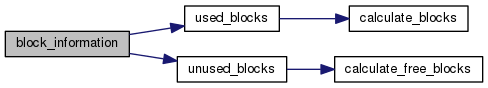
\includegraphics[width=350pt]{memory_management_8h_a9961d9a3b8f1cab8d2801a51cac018c1_cgraph}
\end{center}
\end{figure}




Here is the caller graph for this function\+:
\nopagebreak
\begin{figure}[H]
\begin{center}
\leavevmode
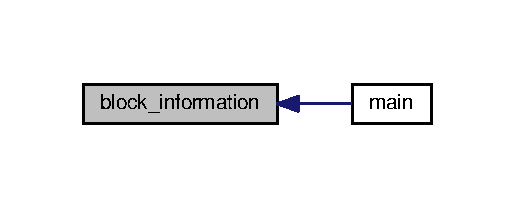
\includegraphics[width=247pt]{memory_management_8h_a9961d9a3b8f1cab8d2801a51cac018c1_icgraph}
\end{center}
\end{figure}


\hypertarget{memory_management_8h_ab62a2cbf81f6577db0668f46aed364ef}{}\index{memory\+Management.\+h@{memory\+Management.\+h}!calculate\+\_\+blocks@{calculate\+\_\+blocks}}
\index{calculate\+\_\+blocks@{calculate\+\_\+blocks}!memory\+Management.\+h@{memory\+Management.\+h}}
\paragraph[{calculate\+\_\+blocks}]{\setlength{\rightskip}{0pt plus 5cm}int calculate\+\_\+blocks (
\begin{DoxyParamCaption}
\item[{int}]{minimum, }
\item[{int}]{maximum}
\end{DoxyParamCaption}
)}\label{memory_management_8h_ab62a2cbf81f6577db0668f46aed364ef}


Here is the caller graph for this function\+:
\nopagebreak
\begin{figure}[H]
\begin{center}
\leavevmode
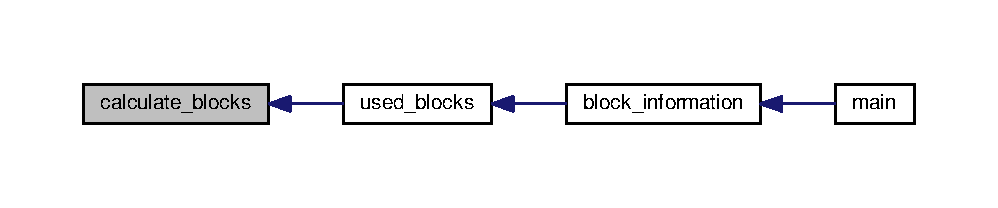
\includegraphics[width=350pt]{memory_management_8h_ab62a2cbf81f6577db0668f46aed364ef_icgraph}
\end{center}
\end{figure}


\hypertarget{memory_management_8h_a156fe06c8c22c3783995e8c2ea0621b9}{}\index{memory\+Management.\+h@{memory\+Management.\+h}!calculate\+\_\+free\+\_\+blocks@{calculate\+\_\+free\+\_\+blocks}}
\index{calculate\+\_\+free\+\_\+blocks@{calculate\+\_\+free\+\_\+blocks}!memory\+Management.\+h@{memory\+Management.\+h}}
\paragraph[{calculate\+\_\+free\+\_\+blocks}]{\setlength{\rightskip}{0pt plus 5cm}int calculate\+\_\+free\+\_\+blocks (
\begin{DoxyParamCaption}
\item[{int}]{minimum, }
\item[{int}]{maximum}
\end{DoxyParamCaption}
)}\label{memory_management_8h_a156fe06c8c22c3783995e8c2ea0621b9}


Here is the caller graph for this function\+:
\nopagebreak
\begin{figure}[H]
\begin{center}
\leavevmode
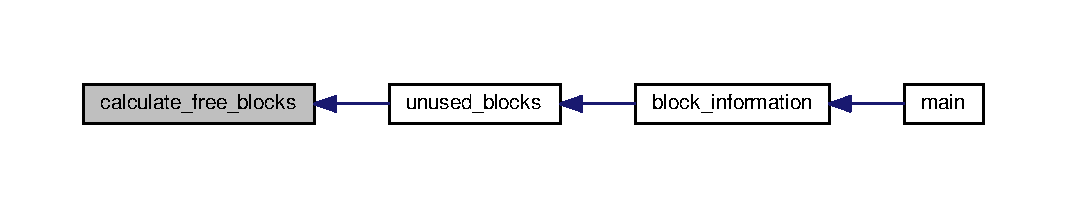
\includegraphics[width=350pt]{memory_management_8h_a156fe06c8c22c3783995e8c2ea0621b9_icgraph}
\end{center}
\end{figure}


\hypertarget{memory_management_8h_aea43d1dfada1be33a518865f1dfec034}{}\index{memory\+Management.\+h@{memory\+Management.\+h}!check\+\_\+for\+\_\+space@{check\+\_\+for\+\_\+space}}
\index{check\+\_\+for\+\_\+space@{check\+\_\+for\+\_\+space}!memory\+Management.\+h@{memory\+Management.\+h}}
\paragraph[{check\+\_\+for\+\_\+space}]{\setlength{\rightskip}{0pt plus 5cm}void$\ast$ check\+\_\+for\+\_\+space (
\begin{DoxyParamCaption}
\item[{int}]{size}
\end{DoxyParamCaption}
)}\label{memory_management_8h_aea43d1dfada1be33a518865f1dfec034}


Here is the call graph for this function\+:
\nopagebreak
\begin{figure}[H]
\begin{center}
\leavevmode
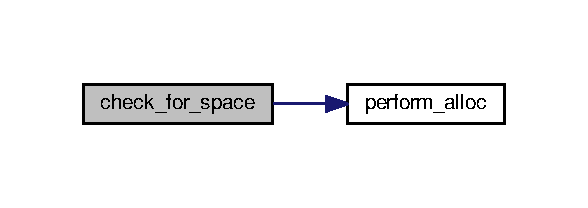
\includegraphics[width=282pt]{memory_management_8h_aea43d1dfada1be33a518865f1dfec034_cgraph}
\end{center}
\end{figure}




Here is the caller graph for this function\+:
\nopagebreak
\begin{figure}[H]
\begin{center}
\leavevmode
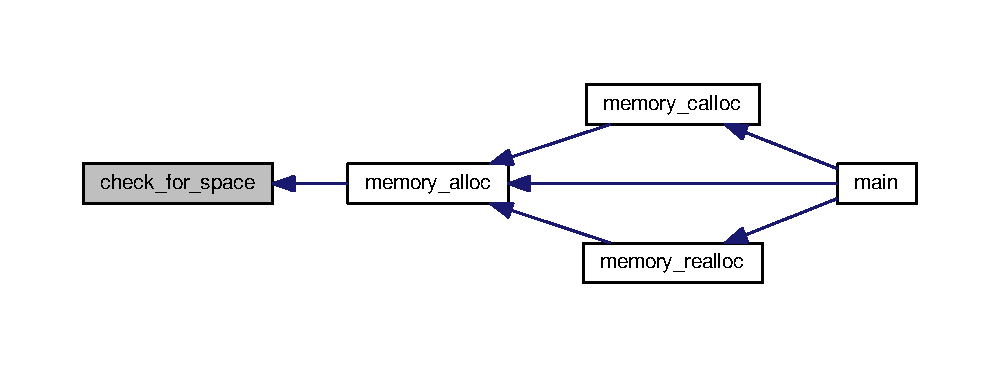
\includegraphics[width=350pt]{memory_management_8h_aea43d1dfada1be33a518865f1dfec034_icgraph}
\end{center}
\end{figure}


\hypertarget{memory_management_8h_a163c8fc7314dff46f38171fe7e652ade}{}\index{memory\+Management.\+h@{memory\+Management.\+h}!delete\+\_\+pointer@{delete\+\_\+pointer}}
\index{delete\+\_\+pointer@{delete\+\_\+pointer}!memory\+Management.\+h@{memory\+Management.\+h}}
\paragraph[{delete\+\_\+pointer}]{\setlength{\rightskip}{0pt plus 5cm}{\bf status} delete\+\_\+pointer (
\begin{DoxyParamCaption}
\item[{int}]{minimum, }
\item[{int}]{start, }
\item[{int}]{size, }
\item[{void $\ast$}]{ptr}
\end{DoxyParamCaption}
)}\label{memory_management_8h_a163c8fc7314dff46f38171fe7e652ade}


Here is the caller graph for this function\+:
\nopagebreak
\begin{figure}[H]
\begin{center}
\leavevmode
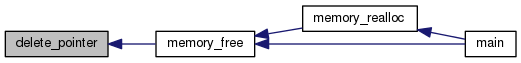
\includegraphics[width=350pt]{memory_management_8h_a163c8fc7314dff46f38171fe7e652ade_icgraph}
\end{center}
\end{figure}


\hypertarget{memory_management_8h_a088ff8aff3fbfc997ad69afced4574c8}{}\index{memory\+Management.\+h@{memory\+Management.\+h}!free\+\_\+block\+\_\+information@{free\+\_\+block\+\_\+information}}
\index{free\+\_\+block\+\_\+information@{free\+\_\+block\+\_\+information}!memory\+Management.\+h@{memory\+Management.\+h}}
\paragraph[{free\+\_\+block\+\_\+information}]{\setlength{\rightskip}{0pt plus 5cm}{\bf status} free\+\_\+block\+\_\+information (
\begin{DoxyParamCaption}
\item[{void}]{}
\end{DoxyParamCaption}
)}\label{memory_management_8h_a088ff8aff3fbfc997ad69afced4574c8}
\hypertarget{memory_management_8h_ae30a35d507593a3635856b601305dd38}{}\index{memory\+Management.\+h@{memory\+Management.\+h}!memory\+\_\+alloc@{memory\+\_\+alloc}}
\index{memory\+\_\+alloc@{memory\+\_\+alloc}!memory\+Management.\+h@{memory\+Management.\+h}}
\paragraph[{memory\+\_\+alloc}]{\setlength{\rightskip}{0pt plus 5cm}void$\ast$ memory\+\_\+alloc (
\begin{DoxyParamCaption}
\item[{int}]{size}
\end{DoxyParamCaption}
)}\label{memory_management_8h_ae30a35d507593a3635856b601305dd38}


Here is the call graph for this function\+:
\nopagebreak
\begin{figure}[H]
\begin{center}
\leavevmode
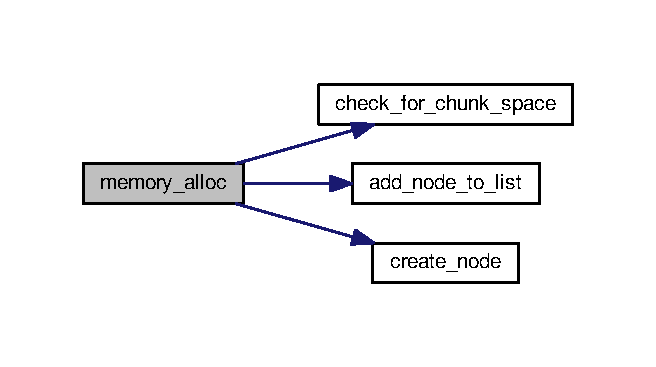
\includegraphics[width=350pt]{memory_management_8h_ae30a35d507593a3635856b601305dd38_cgraph}
\end{center}
\end{figure}




Here is the caller graph for this function\+:
\nopagebreak
\begin{figure}[H]
\begin{center}
\leavevmode
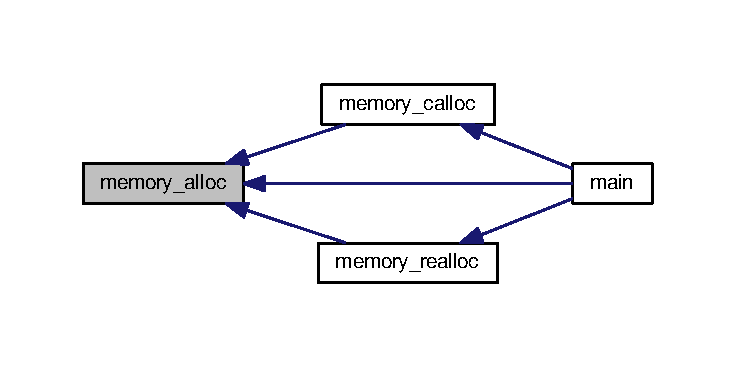
\includegraphics[width=350pt]{memory_management_8h_ae30a35d507593a3635856b601305dd38_icgraph}
\end{center}
\end{figure}


\hypertarget{memory_management_8h_a9fddae3713297adcee22fae422fe4383}{}\index{memory\+Management.\+h@{memory\+Management.\+h}!memory\+\_\+calloc@{memory\+\_\+calloc}}
\index{memory\+\_\+calloc@{memory\+\_\+calloc}!memory\+Management.\+h@{memory\+Management.\+h}}
\paragraph[{memory\+\_\+calloc}]{\setlength{\rightskip}{0pt plus 5cm}void$\ast$ memory\+\_\+calloc (
\begin{DoxyParamCaption}
\item[{int}]{nelem, }
\item[{int}]{elsize}
\end{DoxyParamCaption}
)}\label{memory_management_8h_a9fddae3713297adcee22fae422fe4383}


Here is the call graph for this function\+:
\nopagebreak
\begin{figure}[H]
\begin{center}
\leavevmode
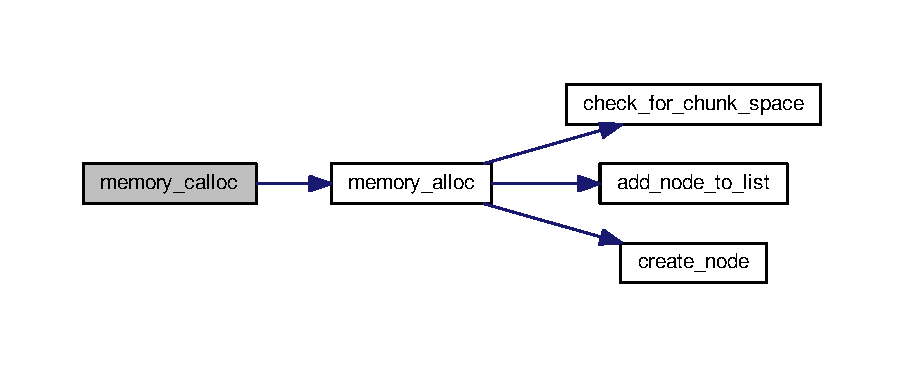
\includegraphics[width=350pt]{memory_management_8h_a9fddae3713297adcee22fae422fe4383_cgraph}
\end{center}
\end{figure}




Here is the caller graph for this function\+:
\nopagebreak
\begin{figure}[H]
\begin{center}
\leavevmode
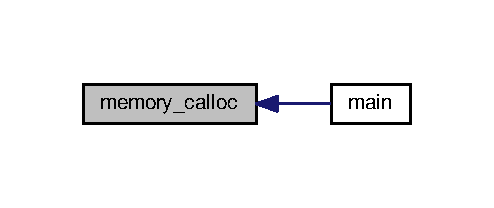
\includegraphics[width=237pt]{memory_management_8h_a9fddae3713297adcee22fae422fe4383_icgraph}
\end{center}
\end{figure}


\hypertarget{memory_management_8h_a8a12d29f1824bf7225965e8b35a0f3a8}{}\index{memory\+Management.\+h@{memory\+Management.\+h}!memory\+\_\+free@{memory\+\_\+free}}
\index{memory\+\_\+free@{memory\+\_\+free}!memory\+Management.\+h@{memory\+Management.\+h}}
\paragraph[{memory\+\_\+free}]{\setlength{\rightskip}{0pt plus 5cm}{\bf status} memory\+\_\+free (
\begin{DoxyParamCaption}
\item[{void $\ast$}]{pointer}
\end{DoxyParamCaption}
)}\label{memory_management_8h_a8a12d29f1824bf7225965e8b35a0f3a8}


Here is the call graph for this function\+:
\nopagebreak
\begin{figure}[H]
\begin{center}
\leavevmode
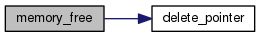
\includegraphics[width=267pt]{memory_management_8h_a8a12d29f1824bf7225965e8b35a0f3a8_cgraph}
\end{center}
\end{figure}




Here is the caller graph for this function\+:
\nopagebreak
\begin{figure}[H]
\begin{center}
\leavevmode
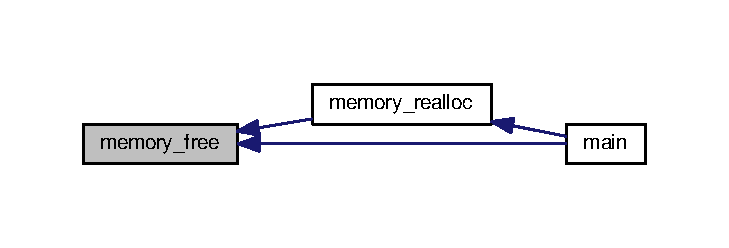
\includegraphics[width=350pt]{memory_management_8h_a8a12d29f1824bf7225965e8b35a0f3a8_icgraph}
\end{center}
\end{figure}


\hypertarget{memory_management_8h_aeae46c0f1bc40e0e3b469f40feefd8d0}{}\index{memory\+Management.\+h@{memory\+Management.\+h}!memory\+\_\+realloc@{memory\+\_\+realloc}}
\index{memory\+\_\+realloc@{memory\+\_\+realloc}!memory\+Management.\+h@{memory\+Management.\+h}}
\paragraph[{memory\+\_\+realloc}]{\setlength{\rightskip}{0pt plus 5cm}void$\ast$ memory\+\_\+realloc (
\begin{DoxyParamCaption}
\item[{void $\ast$}]{ptr, }
\item[{int}]{size}
\end{DoxyParamCaption}
)}\label{memory_management_8h_aeae46c0f1bc40e0e3b469f40feefd8d0}


Here is the call graph for this function\+:
\nopagebreak
\begin{figure}[H]
\begin{center}
\leavevmode
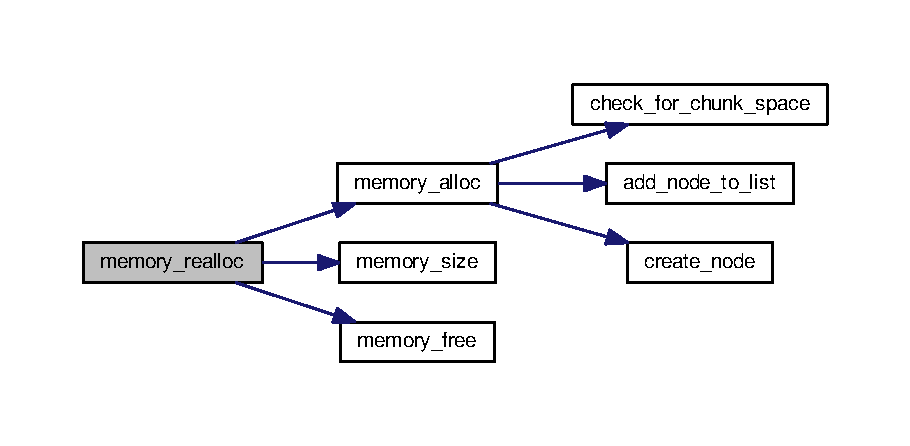
\includegraphics[width=350pt]{memory_management_8h_aeae46c0f1bc40e0e3b469f40feefd8d0_cgraph}
\end{center}
\end{figure}




Here is the caller graph for this function\+:
\nopagebreak
\begin{figure}[H]
\begin{center}
\leavevmode
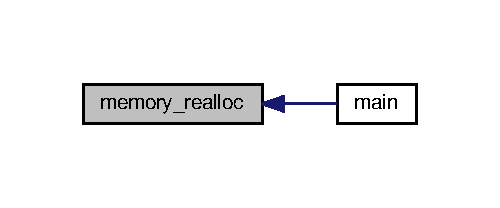
\includegraphics[width=240pt]{memory_management_8h_aeae46c0f1bc40e0e3b469f40feefd8d0_icgraph}
\end{center}
\end{figure}


\hypertarget{memory_management_8h_a3e2309af44a44009e20dea96b76a5f06}{}\index{memory\+Management.\+h@{memory\+Management.\+h}!memory\+\_\+size@{memory\+\_\+size}}
\index{memory\+\_\+size@{memory\+\_\+size}!memory\+Management.\+h@{memory\+Management.\+h}}
\paragraph[{memory\+\_\+size}]{\setlength{\rightskip}{0pt plus 5cm}int memory\+\_\+size (
\begin{DoxyParamCaption}
\item[{void $\ast$}]{ptr}
\end{DoxyParamCaption}
)}\label{memory_management_8h_a3e2309af44a44009e20dea96b76a5f06}


Here is the caller graph for this function\+:
\nopagebreak
\begin{figure}[H]
\begin{center}
\leavevmode
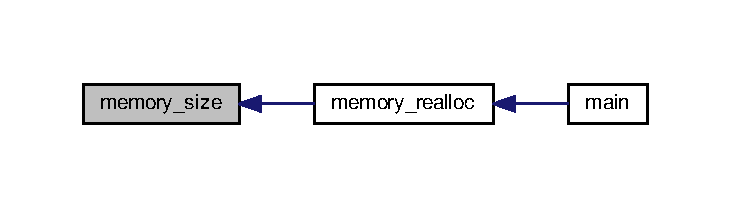
\includegraphics[width=350pt]{memory_management_8h_a3e2309af44a44009e20dea96b76a5f06_icgraph}
\end{center}
\end{figure}


\hypertarget{memory_management_8h_aaa1cfd5c78cb649d31cdcf5056523f9c}{}\index{memory\+Management.\+h@{memory\+Management.\+h}!perform\+\_\+alloc@{perform\+\_\+alloc}}
\index{perform\+\_\+alloc@{perform\+\_\+alloc}!memory\+Management.\+h@{memory\+Management.\+h}}
\paragraph[{perform\+\_\+alloc}]{\setlength{\rightskip}{0pt plus 5cm}int perform\+\_\+alloc (
\begin{DoxyParamCaption}
\item[{int}]{minimum, }
\item[{int}]{maximum, }
\item[{int}]{start, }
\item[{int}]{size}
\end{DoxyParamCaption}
)}\label{memory_management_8h_aaa1cfd5c78cb649d31cdcf5056523f9c}


Here is the caller graph for this function\+:
\nopagebreak
\begin{figure}[H]
\begin{center}
\leavevmode
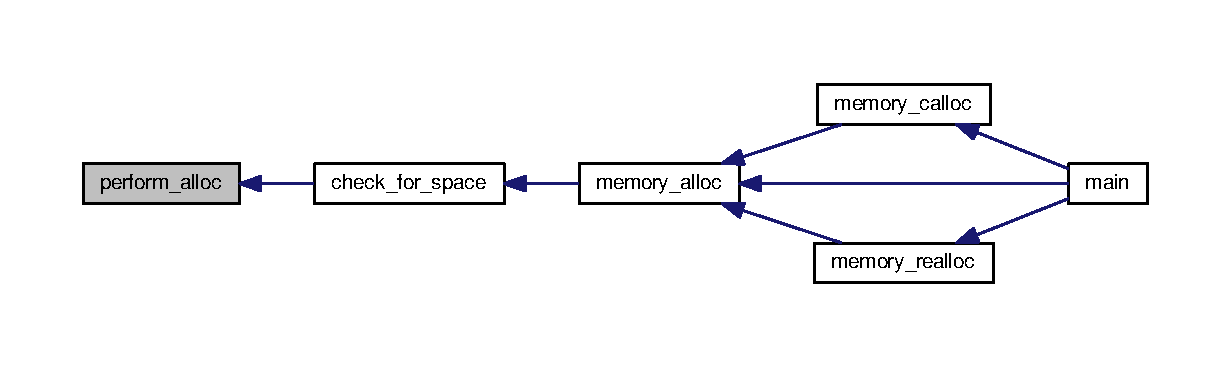
\includegraphics[width=350pt]{memory_management_8h_aaa1cfd5c78cb649d31cdcf5056523f9c_icgraph}
\end{center}
\end{figure}


\hypertarget{memory_management_8h_a84a886fa82e1e3db2ab9e16c3a3b1434}{}\index{memory\+Management.\+h@{memory\+Management.\+h}!unused\+\_\+blocks@{unused\+\_\+blocks}}
\index{unused\+\_\+blocks@{unused\+\_\+blocks}!memory\+Management.\+h@{memory\+Management.\+h}}
\paragraph[{unused\+\_\+blocks}]{\setlength{\rightskip}{0pt plus 5cm}int unused\+\_\+blocks (
\begin{DoxyParamCaption}
\item[{int}]{size}
\end{DoxyParamCaption}
)}\label{memory_management_8h_a84a886fa82e1e3db2ab9e16c3a3b1434}


Here is the call graph for this function\+:
\nopagebreak
\begin{figure}[H]
\begin{center}
\leavevmode
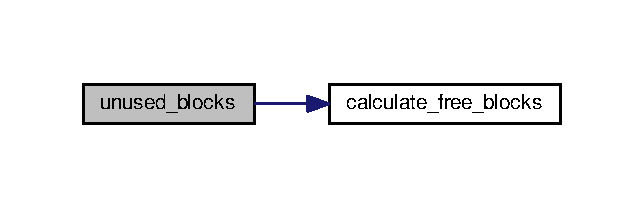
\includegraphics[width=309pt]{memory_management_8h_a84a886fa82e1e3db2ab9e16c3a3b1434_cgraph}
\end{center}
\end{figure}




Here is the caller graph for this function\+:
\nopagebreak
\begin{figure}[H]
\begin{center}
\leavevmode
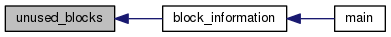
\includegraphics[width=350pt]{memory_management_8h_a84a886fa82e1e3db2ab9e16c3a3b1434_icgraph}
\end{center}
\end{figure}


\hypertarget{memory_management_8h_a8758c4e9207b46696939c497d7688b74}{}\index{memory\+Management.\+h@{memory\+Management.\+h}!used\+\_\+blocks@{used\+\_\+blocks}}
\index{used\+\_\+blocks@{used\+\_\+blocks}!memory\+Management.\+h@{memory\+Management.\+h}}
\paragraph[{used\+\_\+blocks}]{\setlength{\rightskip}{0pt plus 5cm}int used\+\_\+blocks (
\begin{DoxyParamCaption}
\item[{int}]{size}
\end{DoxyParamCaption}
)}\label{memory_management_8h_a8758c4e9207b46696939c497d7688b74}


Here is the call graph for this function\+:
\nopagebreak
\begin{figure}[H]
\begin{center}
\leavevmode
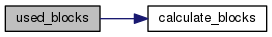
\includegraphics[width=276pt]{memory_management_8h_a8758c4e9207b46696939c497d7688b74_cgraph}
\end{center}
\end{figure}




Here is the caller graph for this function\+:
\nopagebreak
\begin{figure}[H]
\begin{center}
\leavevmode
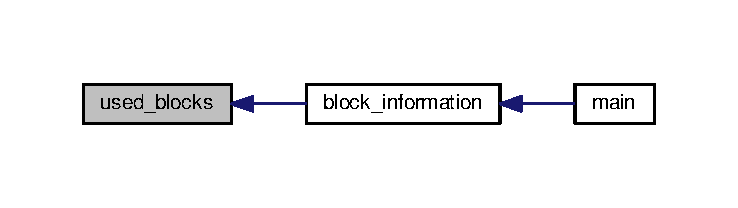
\includegraphics[width=350pt]{memory_management_8h_a8758c4e9207b46696939c497d7688b74_icgraph}
\end{center}
\end{figure}



\hypertarget{memory_management_8c}{}\subsection{src/memory\+Management.c File Reference}
\label{memory_management_8c}\index{src/memory\+Management.\+c@{src/memory\+Management.\+c}}
{\ttfamily \#include $<$stddef.\+h$>$}\\*
{\ttfamily \#include \char`\"{}memory\+Management.\+h\char`\"{}}\\*
Include dependency graph for memory\+Management.\+c\+:
\nopagebreak
\begin{figure}[H]
\begin{center}
\leavevmode
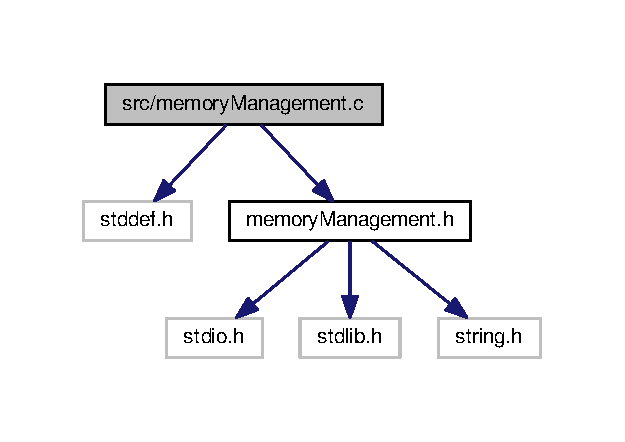
\includegraphics[width=300pt]{memory_management_8c__incl}
\end{center}
\end{figure}
\subsubsection*{Functions}
\begin{DoxyCompactItemize}
\item 
void $\ast$ \hyperlink{memory_management_8c_ae30a35d507593a3635856b601305dd38}{memory\+\_\+alloc} (int size)
\item 
\hyperlink{memory_management_8h_a015eb90e0de9f16e87bd149d4b9ce959}{status} \hyperlink{memory_management_8c_ae134f9f03edd9c11c52eb9e3887911da}{add\+\_\+node\+\_\+to\+\_\+list} (struct \hyperlink{memory_management_8h_struct__info__area}{\+\_\+info\+\_\+area} $\ast$new\+Node)
\item 
struct \hyperlink{memory_management_8h_struct__info__area}{\+\_\+info\+\_\+area} $\ast$ \hyperlink{memory_management_8c_ac30901f2f52d2898523245fe4ad744a0}{create\+\_\+node} (int size)
\item 
\hyperlink{memory_management_8h_a015eb90e0de9f16e87bd149d4b9ce959}{status} \hyperlink{memory_management_8c_a4445092804b80242b5a1c124978837e8}{memory\+\_\+information} ()
\item 
\hyperlink{memory_management_8h_a015eb90e0de9f16e87bd149d4b9ce959}{status} \hyperlink{memory_management_8c_a8a12d29f1824bf7225965e8b35a0f3a8}{memory\+\_\+free} (void $\ast$pointer)
\item 
void $\ast$ \hyperlink{memory_management_8c_a0ee12c76feab0bfc62d67af9989f828d}{check\+\_\+for\+\_\+chunk\+\_\+space} (int size)
\item 
void $\ast$ \hyperlink{memory_management_8c_a9fddae3713297adcee22fae422fe4383}{memory\+\_\+calloc} (int nelem, int elsize)
\item 
void $\ast$ \hyperlink{memory_management_8c_aeae46c0f1bc40e0e3b469f40feefd8d0}{memory\+\_\+realloc} (void $\ast$ptr, int size)
\item 
int \hyperlink{memory_management_8c_a401d53c4641dc4f12bc3251d36d1bfe3}{memory\+\_\+size} (void $\ast$pointer)
\item 
\hyperlink{memory_management_8h_a015eb90e0de9f16e87bd149d4b9ce959}{status} \hyperlink{memory_management_8c_a5e16e5d3309afde94b8d6f9fc6f2364a}{display\+\_\+list} ()
\end{DoxyCompactItemize}
\subsubsection*{Variables}
\begin{DoxyCompactItemize}
\item 
\hyperlink{memory_management_8c_a64b0840001d30ff8cd416759a03542ce}{in} = \hyperlink{memory_management_8h_a4d11bc62f87fecb66ddb08bbe922e468}{I\+N\+I\+T\+I\+A\+L\+\_\+\+Z\+E\+R\+O}
\item 
\hyperlink{memory_management_8c_a076f09d09570b6fb22632de428a3ec5e}{area\+Index} = \hyperlink{memory_management_8h_a4d11bc62f87fecb66ddb08bbe922e468}{I\+N\+I\+T\+I\+A\+L\+\_\+\+Z\+E\+R\+O}
\item 
\hyperlink{memory_management_8c_a7d545f1851a11aa5a292886d35957bdc}{size\+Of\+Node} = sizeof( struct \hyperlink{memory_management_8h_struct__info__area}{\+\_\+info\+\_\+area} )
\item 
struct \hyperlink{memory_management_8h_struct__info__area}{\+\_\+info\+\_\+area} $\ast$ \hyperlink{memory_management_8c_a13b95480ca1ec551d303fb6b31b5ee9d}{head} = N\+U\+L\+L
\item 
struct \hyperlink{memory_management_8h_struct__info__area}{\+\_\+info\+\_\+area} $\ast$ \hyperlink{memory_management_8c_addbea52120befa5218ab585272604dd5}{current} = N\+U\+L\+L
\end{DoxyCompactItemize}


\subsubsection{Function Documentation}
\hypertarget{memory_management_8c_ae134f9f03edd9c11c52eb9e3887911da}{}\index{memory\+Management.\+c@{memory\+Management.\+c}!add\+\_\+node\+\_\+to\+\_\+list@{add\+\_\+node\+\_\+to\+\_\+list}}
\index{add\+\_\+node\+\_\+to\+\_\+list@{add\+\_\+node\+\_\+to\+\_\+list}!memory\+Management.\+c@{memory\+Management.\+c}}
\paragraph[{add\+\_\+node\+\_\+to\+\_\+list}]{\setlength{\rightskip}{0pt plus 5cm}{\bf status} add\+\_\+node\+\_\+to\+\_\+list (
\begin{DoxyParamCaption}
\item[{struct {\bf \+\_\+info\+\_\+area} $\ast$}]{new\+Node}
\end{DoxyParamCaption}
)}\label{memory_management_8c_ae134f9f03edd9c11c52eb9e3887911da}


Here is the caller graph for this function\+:
\nopagebreak
\begin{figure}[H]
\begin{center}
\leavevmode
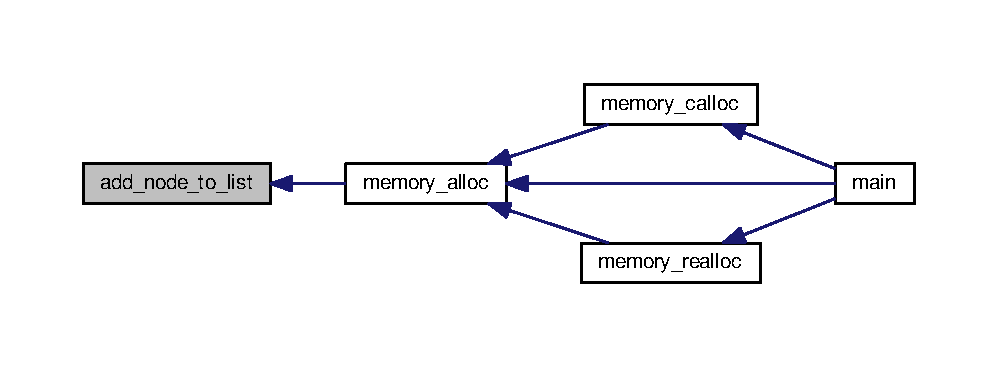
\includegraphics[width=350pt]{memory_management_8c_ae134f9f03edd9c11c52eb9e3887911da_icgraph}
\end{center}
\end{figure}


\hypertarget{memory_management_8c_a0ee12c76feab0bfc62d67af9989f828d}{}\index{memory\+Management.\+c@{memory\+Management.\+c}!check\+\_\+for\+\_\+chunk\+\_\+space@{check\+\_\+for\+\_\+chunk\+\_\+space}}
\index{check\+\_\+for\+\_\+chunk\+\_\+space@{check\+\_\+for\+\_\+chunk\+\_\+space}!memory\+Management.\+c@{memory\+Management.\+c}}
\paragraph[{check\+\_\+for\+\_\+chunk\+\_\+space}]{\setlength{\rightskip}{0pt plus 5cm}void$\ast$ check\+\_\+for\+\_\+chunk\+\_\+space (
\begin{DoxyParamCaption}
\item[{int}]{size}
\end{DoxyParamCaption}
)}\label{memory_management_8c_a0ee12c76feab0bfc62d67af9989f828d}


Here is the caller graph for this function\+:
\nopagebreak
\begin{figure}[H]
\begin{center}
\leavevmode
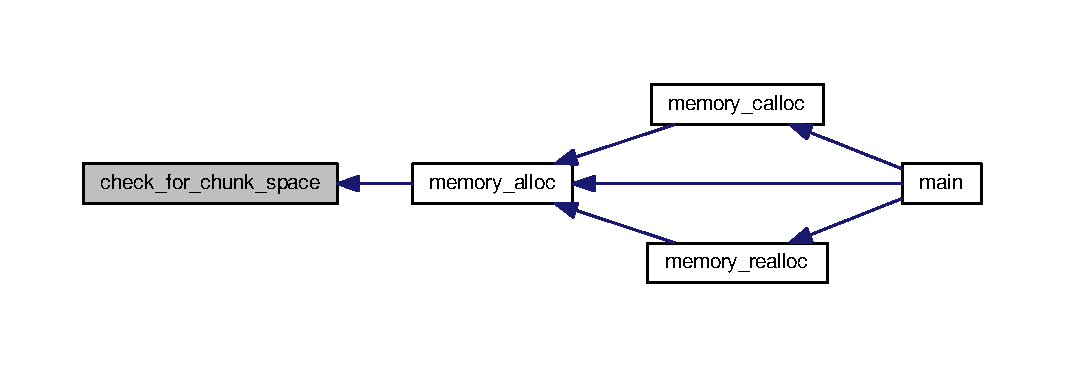
\includegraphics[width=350pt]{memory_management_8c_a0ee12c76feab0bfc62d67af9989f828d_icgraph}
\end{center}
\end{figure}


\hypertarget{memory_management_8c_ac30901f2f52d2898523245fe4ad744a0}{}\index{memory\+Management.\+c@{memory\+Management.\+c}!create\+\_\+node@{create\+\_\+node}}
\index{create\+\_\+node@{create\+\_\+node}!memory\+Management.\+c@{memory\+Management.\+c}}
\paragraph[{create\+\_\+node}]{\setlength{\rightskip}{0pt plus 5cm}struct {\bf \+\_\+info\+\_\+area}$\ast$ create\+\_\+node (
\begin{DoxyParamCaption}
\item[{int}]{size}
\end{DoxyParamCaption}
)}\label{memory_management_8c_ac30901f2f52d2898523245fe4ad744a0}


Here is the caller graph for this function\+:
\nopagebreak
\begin{figure}[H]
\begin{center}
\leavevmode
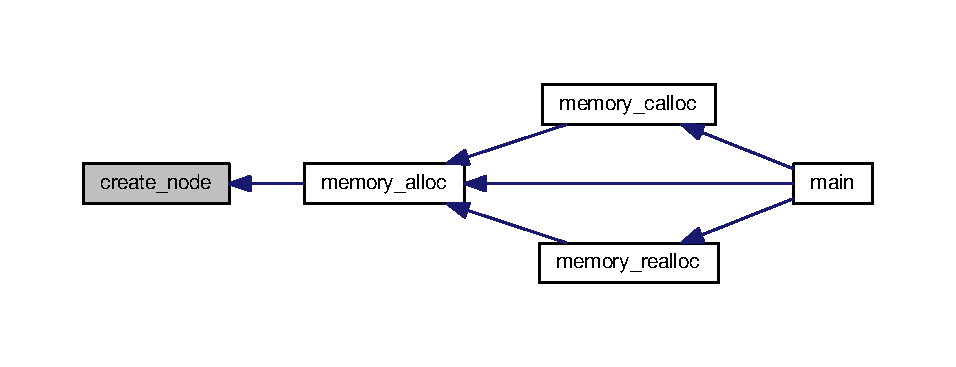
\includegraphics[width=350pt]{memory_management_8c_ac30901f2f52d2898523245fe4ad744a0_icgraph}
\end{center}
\end{figure}


\hypertarget{memory_management_8c_a5e16e5d3309afde94b8d6f9fc6f2364a}{}\index{memory\+Management.\+c@{memory\+Management.\+c}!display\+\_\+list@{display\+\_\+list}}
\index{display\+\_\+list@{display\+\_\+list}!memory\+Management.\+c@{memory\+Management.\+c}}
\paragraph[{display\+\_\+list}]{\setlength{\rightskip}{0pt plus 5cm}{\bf status} display\+\_\+list (
\begin{DoxyParamCaption}
{}
\end{DoxyParamCaption}
)}\label{memory_management_8c_a5e16e5d3309afde94b8d6f9fc6f2364a}


Here is the caller graph for this function\+:
\nopagebreak
\begin{figure}[H]
\begin{center}
\leavevmode
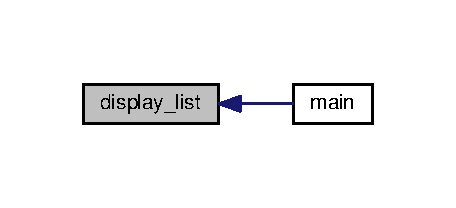
\includegraphics[width=219pt]{memory_management_8c_a5e16e5d3309afde94b8d6f9fc6f2364a_icgraph}
\end{center}
\end{figure}


\hypertarget{memory_management_8c_ae30a35d507593a3635856b601305dd38}{}\index{memory\+Management.\+c@{memory\+Management.\+c}!memory\+\_\+alloc@{memory\+\_\+alloc}}
\index{memory\+\_\+alloc@{memory\+\_\+alloc}!memory\+Management.\+c@{memory\+Management.\+c}}
\paragraph[{memory\+\_\+alloc}]{\setlength{\rightskip}{0pt plus 5cm}void$\ast$ memory\+\_\+alloc (
\begin{DoxyParamCaption}
\item[{int}]{size}
\end{DoxyParamCaption}
)}\label{memory_management_8c_ae30a35d507593a3635856b601305dd38}


Here is the call graph for this function\+:
\nopagebreak
\begin{figure}[H]
\begin{center}
\leavevmode
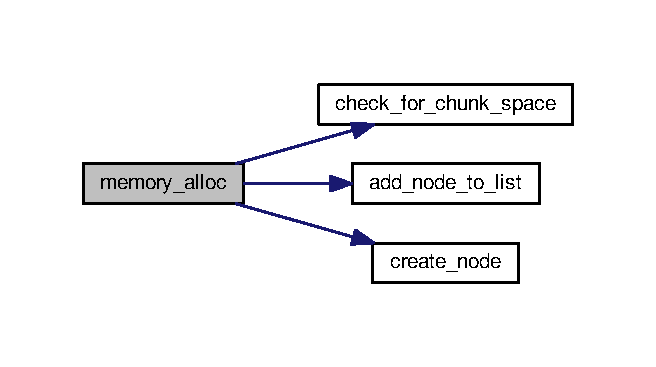
\includegraphics[width=315pt]{memory_management_8c_ae30a35d507593a3635856b601305dd38_cgraph}
\end{center}
\end{figure}




Here is the caller graph for this function\+:
\nopagebreak
\begin{figure}[H]
\begin{center}
\leavevmode
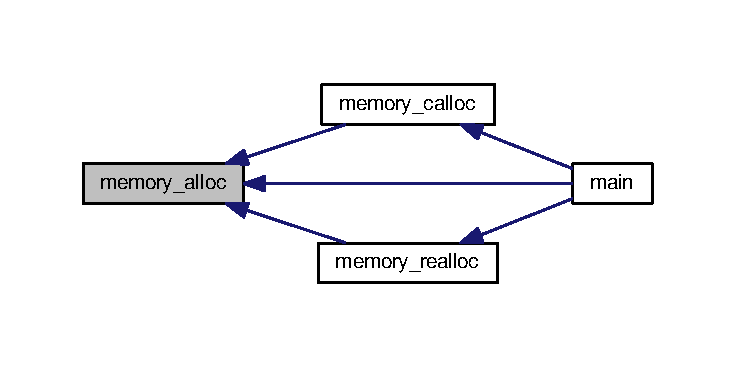
\includegraphics[width=350pt]{memory_management_8c_ae30a35d507593a3635856b601305dd38_icgraph}
\end{center}
\end{figure}


\hypertarget{memory_management_8c_a9fddae3713297adcee22fae422fe4383}{}\index{memory\+Management.\+c@{memory\+Management.\+c}!memory\+\_\+calloc@{memory\+\_\+calloc}}
\index{memory\+\_\+calloc@{memory\+\_\+calloc}!memory\+Management.\+c@{memory\+Management.\+c}}
\paragraph[{memory\+\_\+calloc}]{\setlength{\rightskip}{0pt plus 5cm}void$\ast$ memory\+\_\+calloc (
\begin{DoxyParamCaption}
\item[{int}]{nelem, }
\item[{int}]{elsize}
\end{DoxyParamCaption}
)}\label{memory_management_8c_a9fddae3713297adcee22fae422fe4383}


Here is the call graph for this function\+:
\nopagebreak
\begin{figure}[H]
\begin{center}
\leavevmode
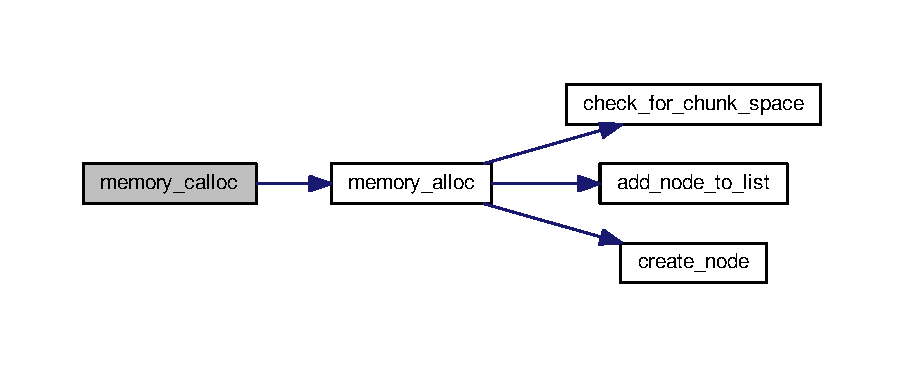
\includegraphics[width=350pt]{memory_management_8c_a9fddae3713297adcee22fae422fe4383_cgraph}
\end{center}
\end{figure}




Here is the caller graph for this function\+:
\nopagebreak
\begin{figure}[H]
\begin{center}
\leavevmode
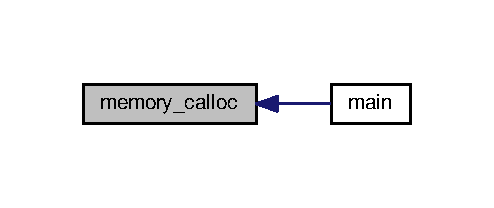
\includegraphics[width=237pt]{memory_management_8c_a9fddae3713297adcee22fae422fe4383_icgraph}
\end{center}
\end{figure}


\hypertarget{memory_management_8c_a8a12d29f1824bf7225965e8b35a0f3a8}{}\index{memory\+Management.\+c@{memory\+Management.\+c}!memory\+\_\+free@{memory\+\_\+free}}
\index{memory\+\_\+free@{memory\+\_\+free}!memory\+Management.\+c@{memory\+Management.\+c}}
\paragraph[{memory\+\_\+free}]{\setlength{\rightskip}{0pt plus 5cm}{\bf status} memory\+\_\+free (
\begin{DoxyParamCaption}
\item[{void $\ast$}]{pointer}
\end{DoxyParamCaption}
)}\label{memory_management_8c_a8a12d29f1824bf7225965e8b35a0f3a8}


Here is the caller graph for this function\+:
\nopagebreak
\begin{figure}[H]
\begin{center}
\leavevmode
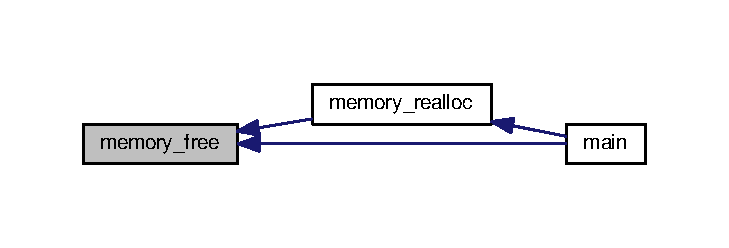
\includegraphics[width=350pt]{memory_management_8c_a8a12d29f1824bf7225965e8b35a0f3a8_icgraph}
\end{center}
\end{figure}


\hypertarget{memory_management_8c_a4445092804b80242b5a1c124978837e8}{}\index{memory\+Management.\+c@{memory\+Management.\+c}!memory\+\_\+information@{memory\+\_\+information}}
\index{memory\+\_\+information@{memory\+\_\+information}!memory\+Management.\+c@{memory\+Management.\+c}}
\paragraph[{memory\+\_\+information}]{\setlength{\rightskip}{0pt plus 5cm}{\bf status} memory\+\_\+information (
\begin{DoxyParamCaption}
{}
\end{DoxyParamCaption}
)}\label{memory_management_8c_a4445092804b80242b5a1c124978837e8}


Here is the caller graph for this function\+:
\nopagebreak
\begin{figure}[H]
\begin{center}
\leavevmode
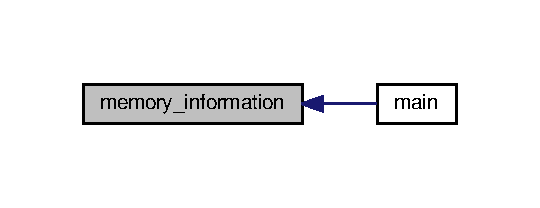
\includegraphics[width=259pt]{memory_management_8c_a4445092804b80242b5a1c124978837e8_icgraph}
\end{center}
\end{figure}


\hypertarget{memory_management_8c_aeae46c0f1bc40e0e3b469f40feefd8d0}{}\index{memory\+Management.\+c@{memory\+Management.\+c}!memory\+\_\+realloc@{memory\+\_\+realloc}}
\index{memory\+\_\+realloc@{memory\+\_\+realloc}!memory\+Management.\+c@{memory\+Management.\+c}}
\paragraph[{memory\+\_\+realloc}]{\setlength{\rightskip}{0pt plus 5cm}void$\ast$ memory\+\_\+realloc (
\begin{DoxyParamCaption}
\item[{void $\ast$}]{ptr, }
\item[{int}]{size}
\end{DoxyParamCaption}
)}\label{memory_management_8c_aeae46c0f1bc40e0e3b469f40feefd8d0}


Here is the call graph for this function\+:
\nopagebreak
\begin{figure}[H]
\begin{center}
\leavevmode
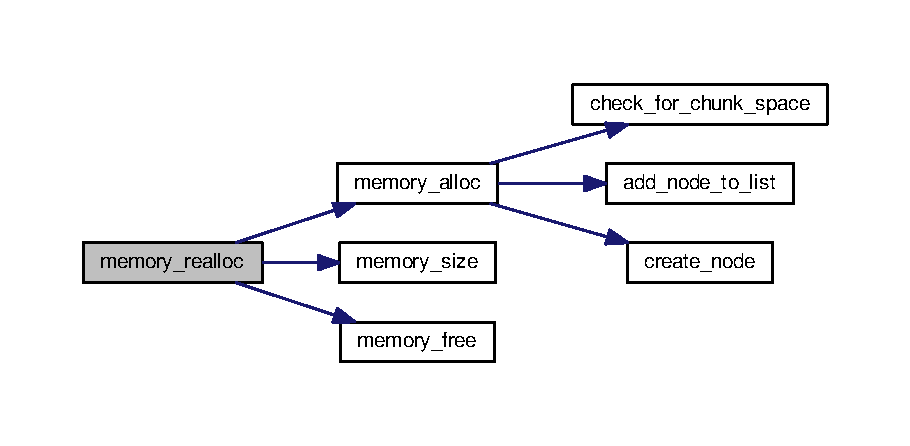
\includegraphics[width=350pt]{memory_management_8c_aeae46c0f1bc40e0e3b469f40feefd8d0_cgraph}
\end{center}
\end{figure}




Here is the caller graph for this function\+:
\nopagebreak
\begin{figure}[H]
\begin{center}
\leavevmode
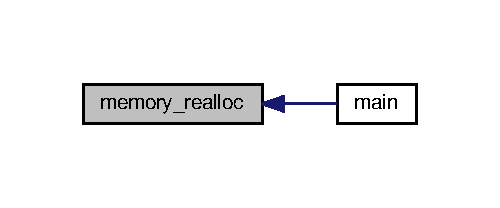
\includegraphics[width=240pt]{memory_management_8c_aeae46c0f1bc40e0e3b469f40feefd8d0_icgraph}
\end{center}
\end{figure}


\hypertarget{memory_management_8c_a401d53c4641dc4f12bc3251d36d1bfe3}{}\index{memory\+Management.\+c@{memory\+Management.\+c}!memory\+\_\+size@{memory\+\_\+size}}
\index{memory\+\_\+size@{memory\+\_\+size}!memory\+Management.\+c@{memory\+Management.\+c}}
\paragraph[{memory\+\_\+size}]{\setlength{\rightskip}{0pt plus 5cm}int memory\+\_\+size (
\begin{DoxyParamCaption}
\item[{void $\ast$}]{pointer}
\end{DoxyParamCaption}
)}\label{memory_management_8c_a401d53c4641dc4f12bc3251d36d1bfe3}


Here is the caller graph for this function\+:
\nopagebreak
\begin{figure}[H]
\begin{center}
\leavevmode
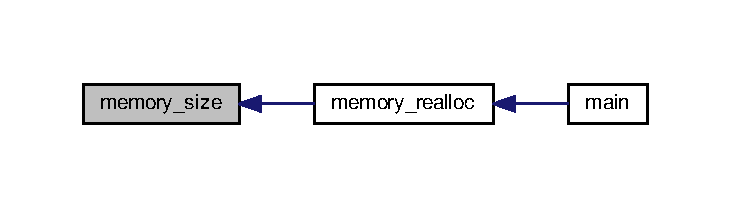
\includegraphics[width=350pt]{memory_management_8c_a401d53c4641dc4f12bc3251d36d1bfe3_icgraph}
\end{center}
\end{figure}




\subsubsection{Variable Documentation}
\hypertarget{memory_management_8c_a076f09d09570b6fb22632de428a3ec5e}{}\index{memory\+Management.\+c@{memory\+Management.\+c}!area\+Index@{area\+Index}}
\index{area\+Index@{area\+Index}!memory\+Management.\+c@{memory\+Management.\+c}}
\paragraph[{area\+Index}]{\setlength{\rightskip}{0pt plus 5cm}area\+Index = {\bf I\+N\+I\+T\+I\+A\+L\+\_\+\+Z\+E\+R\+O}}\label{memory_management_8c_a076f09d09570b6fb22632de428a3ec5e}
\hypertarget{memory_management_8c_addbea52120befa5218ab585272604dd5}{}\index{memory\+Management.\+c@{memory\+Management.\+c}!current@{current}}
\index{current@{current}!memory\+Management.\+c@{memory\+Management.\+c}}
\paragraph[{current}]{\setlength{\rightskip}{0pt plus 5cm}struct {\bf \+\_\+info\+\_\+area} $\ast$ current = N\+U\+L\+L}\label{memory_management_8c_addbea52120befa5218ab585272604dd5}
\hypertarget{memory_management_8c_a13b95480ca1ec551d303fb6b31b5ee9d}{}\index{memory\+Management.\+c@{memory\+Management.\+c}!head@{head}}
\index{head@{head}!memory\+Management.\+c@{memory\+Management.\+c}}
\paragraph[{head}]{\setlength{\rightskip}{0pt plus 5cm}struct {\bf \+\_\+info\+\_\+area}$\ast$ head = N\+U\+L\+L}\label{memory_management_8c_a13b95480ca1ec551d303fb6b31b5ee9d}
\hypertarget{memory_management_8c_a64b0840001d30ff8cd416759a03542ce}{}\index{memory\+Management.\+c@{memory\+Management.\+c}!in@{in}}
\index{in@{in}!memory\+Management.\+c@{memory\+Management.\+c}}
\paragraph[{in}]{\setlength{\rightskip}{0pt plus 5cm}in = {\bf I\+N\+I\+T\+I\+A\+L\+\_\+\+Z\+E\+R\+O}}\label{memory_management_8c_a64b0840001d30ff8cd416759a03542ce}
\hypertarget{memory_management_8c_a7d545f1851a11aa5a292886d35957bdc}{}\index{memory\+Management.\+c@{memory\+Management.\+c}!size\+Of\+Node@{size\+Of\+Node}}
\index{size\+Of\+Node@{size\+Of\+Node}!memory\+Management.\+c@{memory\+Management.\+c}}
\paragraph[{size\+Of\+Node}]{\setlength{\rightskip}{0pt plus 5cm}size\+Of\+Node = sizeof( struct {\bf \+\_\+info\+\_\+area} )}\label{memory_management_8c_a7d545f1851a11aa5a292886d35957bdc}

\hypertarget{user_8c}{}\subsection{src/user.c File Reference}
\label{user_8c}\index{src/user.\+c@{src/user.\+c}}
{\ttfamily \#include \char`\"{}memory\+Management.\+h\char`\"{}}\\*
{\ttfamily \#include $<$stdio.\+h$>$}\\*
{\ttfamily \#include $<$stdlib.\+h$>$}\\*
{\ttfamily \#include $<$time.\+h$>$}\\*
Include dependency graph for user.\+c\+:
\nopagebreak
\begin{figure}[H]
\begin{center}
\leavevmode
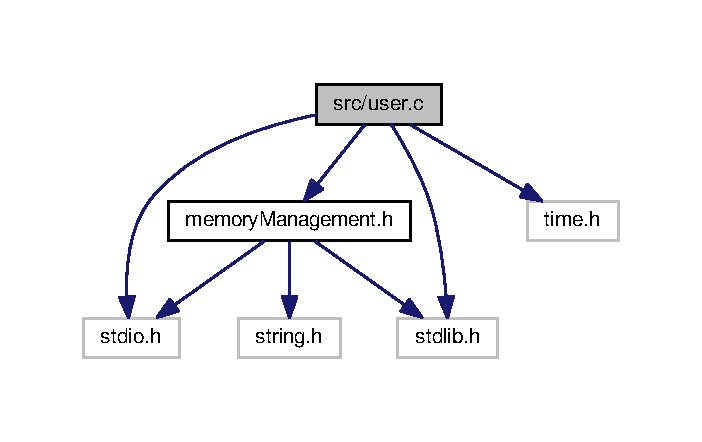
\includegraphics[width=337pt]{user_8c__incl}
\end{center}
\end{figure}
\subsubsection*{Macros}
\begin{DoxyCompactItemize}
\item 
\#define \hyperlink{user_8c_a1719f306508f813a37cd7d28e2c53435}{E\+R\+R\+\_\+\+N\+O\+\_\+\+N\+U\+M}~-\/1
\item 
\#define \hyperlink{user_8c_a6332413b933f27d85c87c288f5b0d260}{E\+R\+R\+\_\+\+N\+O\+\_\+\+M\+E\+M}~-\/2
\item 
\#define \hyperlink{user_8c_a0592dba56693fad79136250c11e5a7fe}{M\+A\+X\+\_\+\+S\+I\+Z\+E}~5000
\item 
\#define \hyperlink{user_8c_a7556679f2a7178d92c14f8f311c592b9}{M\+A\+L\+L\+O\+C\+\_\+\+M\+A\+X\+\_\+\+S\+I\+Z\+E}~2048
\item 
\#define \hyperlink{user_8c_a3f900af529705a735196fabffa13dd66}{C\+A\+L\+L\+O\+C\+\_\+\+M\+A\+X\+\_\+\+S\+I\+Z\+E}~50
\item 
\#define \hyperlink{user_8c_abcb0b28b93251f50ed0d9a89040cda61}{C\+A\+L\+L\+O\+C\+\_\+\+M\+A\+X\+\_\+\+E\+L\+E\+M\+E\+N\+T\+S}~20
\item 
\#define \hyperlink{user_8c_a12b95e73e5048ea0419f593afae7240c}{R\+E\+A\+L\+L\+O\+C\+\_\+\+M\+A\+X\+\_\+\+S\+I\+Z\+E}~2048
\end{DoxyCompactItemize}
\subsubsection*{Functions}
\begin{DoxyCompactItemize}
\item 
int \hyperlink{user_8c_adc26eb8c308ee1308c09c2aab7b8a98e}{my\+Random} (int size)
\item 
int \hyperlink{user_8c_ae66f6b31b5ad750f1fe042a706a4e3d4}{main} ()
\end{DoxyCompactItemize}


\subsubsection{Macro Definition Documentation}
\hypertarget{user_8c_abcb0b28b93251f50ed0d9a89040cda61}{}\index{user.\+c@{user.\+c}!C\+A\+L\+L\+O\+C\+\_\+\+M\+A\+X\+\_\+\+E\+L\+E\+M\+E\+N\+T\+S@{C\+A\+L\+L\+O\+C\+\_\+\+M\+A\+X\+\_\+\+E\+L\+E\+M\+E\+N\+T\+S}}
\index{C\+A\+L\+L\+O\+C\+\_\+\+M\+A\+X\+\_\+\+E\+L\+E\+M\+E\+N\+T\+S@{C\+A\+L\+L\+O\+C\+\_\+\+M\+A\+X\+\_\+\+E\+L\+E\+M\+E\+N\+T\+S}!user.\+c@{user.\+c}}
\paragraph[{C\+A\+L\+L\+O\+C\+\_\+\+M\+A\+X\+\_\+\+E\+L\+E\+M\+E\+N\+T\+S}]{\setlength{\rightskip}{0pt plus 5cm}\#define C\+A\+L\+L\+O\+C\+\_\+\+M\+A\+X\+\_\+\+E\+L\+E\+M\+E\+N\+T\+S~20}\label{user_8c_abcb0b28b93251f50ed0d9a89040cda61}
\hypertarget{user_8c_a3f900af529705a735196fabffa13dd66}{}\index{user.\+c@{user.\+c}!C\+A\+L\+L\+O\+C\+\_\+\+M\+A\+X\+\_\+\+S\+I\+Z\+E@{C\+A\+L\+L\+O\+C\+\_\+\+M\+A\+X\+\_\+\+S\+I\+Z\+E}}
\index{C\+A\+L\+L\+O\+C\+\_\+\+M\+A\+X\+\_\+\+S\+I\+Z\+E@{C\+A\+L\+L\+O\+C\+\_\+\+M\+A\+X\+\_\+\+S\+I\+Z\+E}!user.\+c@{user.\+c}}
\paragraph[{C\+A\+L\+L\+O\+C\+\_\+\+M\+A\+X\+\_\+\+S\+I\+Z\+E}]{\setlength{\rightskip}{0pt plus 5cm}\#define C\+A\+L\+L\+O\+C\+\_\+\+M\+A\+X\+\_\+\+S\+I\+Z\+E~50}\label{user_8c_a3f900af529705a735196fabffa13dd66}
\hypertarget{user_8c_a6332413b933f27d85c87c288f5b0d260}{}\index{user.\+c@{user.\+c}!E\+R\+R\+\_\+\+N\+O\+\_\+\+M\+E\+M@{E\+R\+R\+\_\+\+N\+O\+\_\+\+M\+E\+M}}
\index{E\+R\+R\+\_\+\+N\+O\+\_\+\+M\+E\+M@{E\+R\+R\+\_\+\+N\+O\+\_\+\+M\+E\+M}!user.\+c@{user.\+c}}
\paragraph[{E\+R\+R\+\_\+\+N\+O\+\_\+\+M\+E\+M}]{\setlength{\rightskip}{0pt plus 5cm}\#define E\+R\+R\+\_\+\+N\+O\+\_\+\+M\+E\+M~-\/2}\label{user_8c_a6332413b933f27d85c87c288f5b0d260}
\hypertarget{user_8c_a1719f306508f813a37cd7d28e2c53435}{}\index{user.\+c@{user.\+c}!E\+R\+R\+\_\+\+N\+O\+\_\+\+N\+U\+M@{E\+R\+R\+\_\+\+N\+O\+\_\+\+N\+U\+M}}
\index{E\+R\+R\+\_\+\+N\+O\+\_\+\+N\+U\+M@{E\+R\+R\+\_\+\+N\+O\+\_\+\+N\+U\+M}!user.\+c@{user.\+c}}
\paragraph[{E\+R\+R\+\_\+\+N\+O\+\_\+\+N\+U\+M}]{\setlength{\rightskip}{0pt plus 5cm}\#define E\+R\+R\+\_\+\+N\+O\+\_\+\+N\+U\+M~-\/1}\label{user_8c_a1719f306508f813a37cd7d28e2c53435}
\hypertarget{user_8c_a7556679f2a7178d92c14f8f311c592b9}{}\index{user.\+c@{user.\+c}!M\+A\+L\+L\+O\+C\+\_\+\+M\+A\+X\+\_\+\+S\+I\+Z\+E@{M\+A\+L\+L\+O\+C\+\_\+\+M\+A\+X\+\_\+\+S\+I\+Z\+E}}
\index{M\+A\+L\+L\+O\+C\+\_\+\+M\+A\+X\+\_\+\+S\+I\+Z\+E@{M\+A\+L\+L\+O\+C\+\_\+\+M\+A\+X\+\_\+\+S\+I\+Z\+E}!user.\+c@{user.\+c}}
\paragraph[{M\+A\+L\+L\+O\+C\+\_\+\+M\+A\+X\+\_\+\+S\+I\+Z\+E}]{\setlength{\rightskip}{0pt plus 5cm}\#define M\+A\+L\+L\+O\+C\+\_\+\+M\+A\+X\+\_\+\+S\+I\+Z\+E~2048}\label{user_8c_a7556679f2a7178d92c14f8f311c592b9}
\hypertarget{user_8c_a0592dba56693fad79136250c11e5a7fe}{}\index{user.\+c@{user.\+c}!M\+A\+X\+\_\+\+S\+I\+Z\+E@{M\+A\+X\+\_\+\+S\+I\+Z\+E}}
\index{M\+A\+X\+\_\+\+S\+I\+Z\+E@{M\+A\+X\+\_\+\+S\+I\+Z\+E}!user.\+c@{user.\+c}}
\paragraph[{M\+A\+X\+\_\+\+S\+I\+Z\+E}]{\setlength{\rightskip}{0pt plus 5cm}\#define M\+A\+X\+\_\+\+S\+I\+Z\+E~5000}\label{user_8c_a0592dba56693fad79136250c11e5a7fe}
\hypertarget{user_8c_a12b95e73e5048ea0419f593afae7240c}{}\index{user.\+c@{user.\+c}!R\+E\+A\+L\+L\+O\+C\+\_\+\+M\+A\+X\+\_\+\+S\+I\+Z\+E@{R\+E\+A\+L\+L\+O\+C\+\_\+\+M\+A\+X\+\_\+\+S\+I\+Z\+E}}
\index{R\+E\+A\+L\+L\+O\+C\+\_\+\+M\+A\+X\+\_\+\+S\+I\+Z\+E@{R\+E\+A\+L\+L\+O\+C\+\_\+\+M\+A\+X\+\_\+\+S\+I\+Z\+E}!user.\+c@{user.\+c}}
\paragraph[{R\+E\+A\+L\+L\+O\+C\+\_\+\+M\+A\+X\+\_\+\+S\+I\+Z\+E}]{\setlength{\rightskip}{0pt plus 5cm}\#define R\+E\+A\+L\+L\+O\+C\+\_\+\+M\+A\+X\+\_\+\+S\+I\+Z\+E~2048}\label{user_8c_a12b95e73e5048ea0419f593afae7240c}


\subsubsection{Function Documentation}
\hypertarget{user_8c_ae66f6b31b5ad750f1fe042a706a4e3d4}{}\index{user.\+c@{user.\+c}!main@{main}}
\index{main@{main}!user.\+c@{user.\+c}}
\paragraph[{main}]{\setlength{\rightskip}{0pt plus 5cm}int main (
\begin{DoxyParamCaption}
{}
\end{DoxyParamCaption}
)}\label{user_8c_ae66f6b31b5ad750f1fe042a706a4e3d4}


Here is the call graph for this function\+:
\nopagebreak
\begin{figure}[H]
\begin{center}
\leavevmode
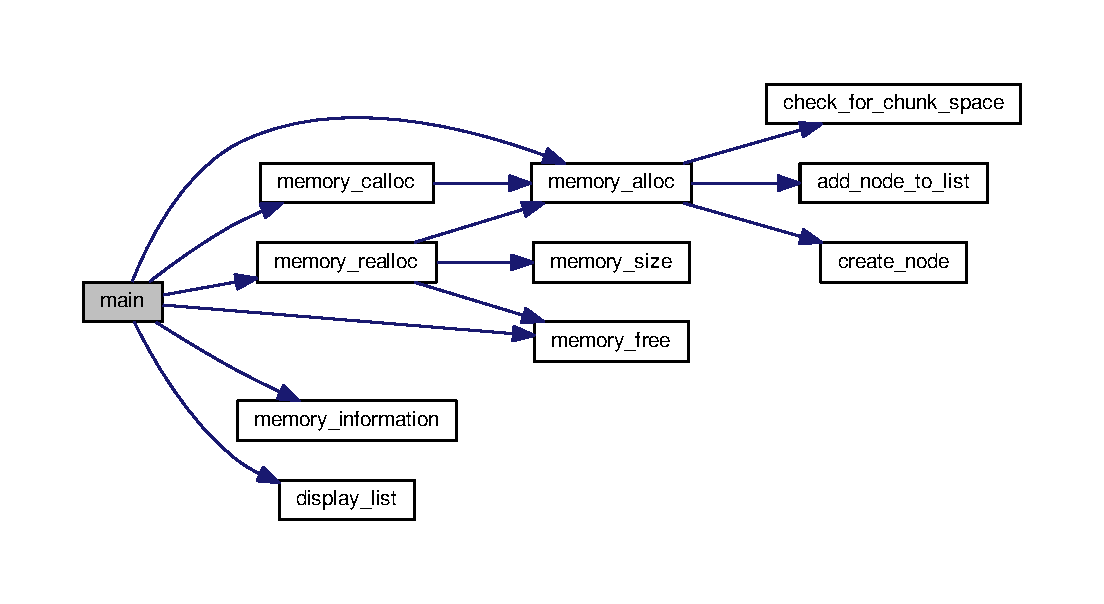
\includegraphics[width=350pt]{user_8c_ae66f6b31b5ad750f1fe042a706a4e3d4_cgraph}
\end{center}
\end{figure}


\hypertarget{user_8c_adc26eb8c308ee1308c09c2aab7b8a98e}{}\index{user.\+c@{user.\+c}!my\+Random@{my\+Random}}
\index{my\+Random@{my\+Random}!user.\+c@{user.\+c}}
\paragraph[{my\+Random}]{\setlength{\rightskip}{0pt plus 5cm}int my\+Random (
\begin{DoxyParamCaption}
\item[{int}]{size}
\end{DoxyParamCaption}
)}\label{user_8c_adc26eb8c308ee1308c09c2aab7b8a98e}

%--- End generated contents ---

% Index
\newpage
\phantomsection
\clearemptydoublepage
\addcontentsline{toc}{section}{Index}
\printindex

\end{document}
